\documentclass[11pt,twoside,a4paper,fleqn]{book} 

%--- Packages to use
%
\usepackage[]{fancyhdr}   
\usepackage[]{natbib}
\usepackage{alltt}
\usepackage{times}
\usepackage{verbatim}
\usepackage{lscape}         % landscape mode of a single page
\usepackage[]{longtable}    % allow tables longer than one page
\usepackage{makeidx}        % index of terms
\usepackage{tabularx}       % allows line breaking in table columns
\usepackage{ifpdf}
\usepackage{fancyvrb}
\usepackage{wrapfig}
\usepackage{url}
\usepackage{amsmath}
\usepackage{xifthen}
\usepackage[T1]{fontenc} 
\usepackage{cprotect}

%--- Margins
%
\voffset-2.0cm
\headheight16pt
\headsep1.1cm
\textheight22cm
\hoffset-1.3cm
\oddsidemargin2.2cm
\textwidth14.0cm
\parskip1ex
\parindent0ex

%--- Headings
%
\pagestyle{fancy}
\renewcommand{\chaptermark}[1]{\markboth{#1}{}}
\renewcommand{\sectionmark}[1]{\markright{\thesection\ #1}}
\fancyhf{}
\fancyhead[LE,RO]{\small{\sc\thepage}}
\fancyhead[LO]{\small{\scshape\rightmark}}
\fancyhead[RE]{\small{\scshape\leftmark}}
\renewcommand{\headrulewidth}{0.5pt}
\renewcommand{\footrulewidth}{0pt}
\fancypagestyle{plain}{%
  \fancyhead{}
  \renewcommand{\headrulewidth}{0pt}
}  


%--- Some layout commands
%
\sloppy
\raggedbottom
\hbadness=10000
\makeindex
\bibliographystyle{egu}
\newcommand{\HRule}{\rule{\linewidth}{0.5mm}} 


%--- PDF/LaTeX specific options
\ifpdf
  \usepackage[pdftex]{graphicx}    % includegraphics
  \DeclareGraphicsExtensions{.pdf}
  \usepackage{color}
  \definecolor{DarkBlue}{rgb}{0,0,0.5}
  \usepackage
    [pdftex,                         % or dvips
     colorlinks=true,
     linkcolor=DarkBlue,
     citecolor=DarkBlue,
     urlcolor=DarkBlue,
     pdftitle={libRadtran User's Guide},
     pdfauthor={B. Mayer, A. Kylling, C. Emde, U. Hamann, R.Buras, J. Gasteiger and B. Richter},
     pdfsubject={},
     pdfkeywords={},
     bookmarks=true,
     bookmarksopen=false,
     pdfpagemode=None,
     plainpages=false,
     pdfpagelabels]
  {hyperref}
  \setcounter{tocdepth}{2}
\else
  \usepackage[dvips]{graphicx}    % includegraphics
  \DeclareGraphicsExtensions{.eps}
  \setcounter{tocdepth}{1}
\fi

\title{libRadtran User's Guide}
\author{Bernhard Mayer, Arve Kylling, Claudia Emde,
  Robert Buras, Ulrich Hamann, Josef Gasteiger, Bettina Richter}

\newcommand{\code}[1]{%
  {\texttt{#1}}}
\newcommand{\fcode}[1]{%
  \ \\[1.5ex]
  \framebox[13cm][l]{
    \begin{minipage}{13cm}
      \small\texttt{#1}
    \end{minipage}
  }
  \ \\
}
  
%aky20100302  {\small\texttt{#1}}}
\newcommand{\file}[1]{%
  {\texttt{#1}}}
%aky20100302  {\small\texttt{#1}}}
\newcommand{\strong}[1]{%
  \textbf{#1}}

%--- Email adresses
\newcommand{\email}[1]{%
  {\small \texttt{#1}}}


%--- For FIXMEs
\newcommand{\FIXME}[1]{{\bfseries FIXME: #1}}

%--- To include example files
\newcommand{\efile}[1]{%
  \fvset{fontsize=\footnotesize, frame=single, fontfamily=courier, samepage=true}%
  \VerbatimInput{#1}%
}

%--- To specify options in uvspec_lex.l / mie_lex.l
\newcommand{\option}[1]{%
\item[#1] \index{#1} \hfill\\} 

%--- To specify parameter in uvspec_lex.l / mie_lex.l
\newcommand{\parameter}[1]{%
\item[#1] \hfill\\} 

%--- specify option in text and create index entry 
\newcommand{\codeidx}[1]{%
  \code{#1}\index{#1}}

%--- MYSTIC documentation 
\newcommand{\ifmystic}[1]{%
  \ifthenelse{\boolean{mystic_doc}}{#1}{}}

%--- MYSTIC3D documentation 
%--- The % at the end of the first line is required; otherwise 
%--- an extra blank was added to the text if threedmystic was FALSE
\newcommand{\ifthreedmystic}[1]{%
  \ifthenelse{\boolean{mystic3d_doc}}{#1}{}}
\cMakeRobust{\ifthreedmystic}

%--- LIDAR documentation (and HIDDEN stuff)
\newcommand{\iflidar}[1]{%
  \ifthenelse{\boolean{lidar_doc}}{#1}{}}

%--- Undocumented options
\newcommand{\undocumented}[1]{%
  \ifthenelse{\boolean{udoc}}{#1}{}}

\newboolean{mystic_doc}
\newboolean{mystic3d_doc}
\newboolean{lidar_doc}
\newboolean{udoc}

\begin{document}

\subsection{Three-dimensional RTE solver \index{MYSTIC} (mystic)} 
\label{sec:mystic}

The Monte Carlo method is the most straightforward way to calculate 
(polarized) radiative transfer. In forward tracing mode  
individual photons are traced on their random paths through the atmosphere.
Starting from top of the atmosphere (for solar radiation), or being thermally
emitted by the atmosphere or surface, the photons are followed until they
hit the surface or leave again at top of the atmosphere (TOA). For
solar radiation, the start position is either a random location in the
TOA plane, with the direction determined by the solar zenith and
azimuth. Originally, the ``Monte Carlo for the physically correct tracing of
photons in cloudy atmospheres'' MYSTIC \citep{mayer2009} has been developed as
a forward tracing method for the calculation of irradiances and radiances in
\ifthreedmystic{3D} plane-parallel atmospheres. Later the model has been extended to fully
spherical geometry and a backward tracing mode \citep{emde2007}. The backward
photon tracing option speeds up the calculation of radiances and allows very
fast calculations in the thermal spectral range.  

\ifthreedmystic{MYSTIC handles three-dimensional water and ice clouds in a
one-dimensional background  atmosphere of molecular scatterers and
absorbers and aerosol particles.  MYSTIC also allows topography as well as 
inhomogeneous surface albedo and BRDF to be considered.}

MYSTIC is now a full vector code: It can handle polarization and
polarization-dependent scattering by randomly oriented particles,
i.e. clouds droplets and particles, aerosol particles, and molecules
\citep{emde2010}. To keep the computational time reasonable for
accurate calculations of e.g. polarized radiances in cloudy
atmospheres several ``tricks'' are required to speed up the
calculations. The first is the so called ``local estimate method''
\citep{marshak2005}. Using this method a photon contributes to the
final result of the calculation each time it is scattered. However, in
the presence of particles with strong forward scattering in the
simulated scene, such as clouds and large aerosols, the local estimate
method will produce so-called ``spikes'', these are rare photons whose
very large contribution to the result leads to slow convergence. The spike
problem can be resolved by using the ``Variance Reduction Optimal
Options Method'' \citep[VROOM,][]{buras2011a}, a collection of several
variance reduction methods which change the photon paths such that the
spikes disappear, but without altering the result (i.e.~the variance
reduction is ``unbiased'').

A detailed introduction to the Monte Carlo technique and in particular
to MYSTIC is given in \citet{mayer2009}. For specific questions 
concerning the Monte Carlo technique the reader is referred to the literature  
\citep{marchuk1980,collins1972,marshak2005,cahalan2005}.

MYSTIC is switched on by the option \code{rte\_solver mystic}. If no
other options are specified MYSTIC computes unpolarized quantities for
a \ifthreedmystic{3D} plane-parallel
atmosphere\ifthreedmystic{~(domain is divided into block-shaped 
boxes)}. If \codeidx{mc\_polarisation} is specified, polarized
quantities are computed. The option \codeidx{mc\_spherical 1D} enables
calculations in a 1D spherical model atmosphere. All MYSTIC-specific
options start with \code{mc\_} and
are described in detail in section~\ref{sec:uvspec_options}.

\ifthreedmystic{
MYSTIC may be provided with various 2D and 3D input files, in addition 
to the standard 1D input files of {\sl uvspec}. The input files may
include the following data:
\begin{itemize}
\item 3D water clouds
\item 3D ice clouds
\item 2D surface albedo
\item 2D elevation
\item 2D BRDF
%\item Lasers and detectors for lidar 
\end{itemize}

If none of these are specified, MYSTIC does basically a 1D calculation
and should compare well with other solvers, in particular \code{disort2}.

MYSTIC operates in a user-defined model-domain. Since periodic boundary 
conditions are applied, the user has to make sure that the quantity to be 
calculated is not affected by the boundaries. For maximum flexibility, 
the different grids (sample, cloud, elevation, albedo or BRDF) are 
completely independent. The only constraint is that the domain size
is equal for all grids used. E.g., clouds may be defined in 5x5x2~km$^3$ 
cubes while the surface albedo is defined on a 1x1~km$^2$ grid, 
the elevation on a 0.1x0.2~km$^2$ grid, and the output might 
be sampled on a 3x4~km$^2$ grid. The only restrictions are 
the available memory, the processor speed, and the requirements on 
the precision of the result (see section~\ref{sec:mc_memory}).

The sampling information for MYSTIC is defined in the input file (e.g.
with \codeidx{mc\_sample\_grid}, \codeidx{zout}, \codeidx{umu}, ...).
After initialization MYSTIC reports how it interpreted the input parameters 
which gives the user a chance to see if it really does what it is 
supposed to be doing.


\subsubsection{Three-dimensional clouds}

The options \codeidx{wc\_file 3D}
and \codeidx{ic\_file 3D} may be used to define 3D water and ice
cloud properties respectively. The model atmosphere may contain both 3D 
(defined in a \code{wc\_file/ic\_file 3D}) and 1D clouds (defined in a 
\code{wc\_file/ic\_file 1D}), but for obvious reasons not in the same layer. The format
of the files is explained in section~\ref{sec:uvspec_options}. 

The conversion from microphysical to optical properties 
is done identically for 1D and 3D clouds and is defined 
by the options \codeidx{wc\_properties} and \codeidx{ic\_properties}. All
possible settings for \code{wc\_properties} and \code{ic\_properties}
have been implemented in MYSTIC (e.g., hu, mie, yang, HEY, baum ...).
The following example shows the easiest possible 3D 
cloud file which defines a checkerboard grid of clouds:
\begin{Verbatim}[fontsize=\footnotesize, frame=single, samepage=true]
  2 2 5 3
  1.0 1.0 0 1 2 3 4 5 

  1 1 2 0.1 10
  2 2 2 0.1 10
\end{Verbatim}
For the layer between 1 and 2 km a 3D cloud is defined with liquid water
content 0.1 $g/m^3$ and effective radius 10 $\mu$m for horizontal 
boxes (1,1) and (2,2). Boxes (1,2) and (2,1) are cloudless. The result are
cubic clouds with a volume of 1x1x1~km$^3$. The microphysical properties are
converted to optical properties according to \code{wc\_properties}.  

\subsubsection{Two-dimensional surface albedo}

A 2D surface albedo may be defined using the option
\codeidx{mc\_albedo\_file}. The format of the file is explained in
section~\ref{sec:uvspec_options}. 

\subsubsection{Topography}

A 2D elevation may be defined using the option 
\codeidx{mc\_elevation\_file}. The ASCII format is explained in
section~\ref{sec:uvspec_options}. For the netcdf format please refer
to \file{README.MC}. 

Caution:
\begin{itemize}
\item To avoid confusion, do not specify an \code{altitude} different
  from 0 in the uvspec input file.
\item There may be problems if the 2D surface hits 0 
  (more testing required). Use 0.001 as lowest altitude.
\item  The elevation file MUST BE PERIODIC
\end{itemize}

Between the grid points, the surface is interpolated 
bilinearely: 
\begin{equation}
  z(x,y) = a + bx + cy + dxy
\end{equation}
where $z$ is the altitude and the coefficients $a$, $b$, $c$, and $d$
are determined from 
the altitudes specified at the four corners of each pixel.
Slant surfaces are treated as they should be; e.g., photons
may be reflected downward at snow-covered mountain sides.

\subsubsection{Bidirectional reflectance distribution function}
MYSTIC allows different homogenous or 2D-inhomogeneous BRDFs. The 
implementation of the different BRDFs is rather heterogeneous,   
as were the requirements when each of them was first implemented.
Please note that BRDFs currently do not work together with topography. The 
very simple reason for that is in structured terrain reflection 
polar angles larger than 90 degree are possible for which the 
existing parameterizations do not provide data. The following  
parameterizations are included:
\begin{itemize}
\item Water BRDF by \citet{cox54a,cox54b}; currently only homogeneous; switched 
  on with \codeidx{brdf\_cam u10}, ... like in the 1D case
\item AMBRALS (Algorithm for Modeling[MODIS] Bidirectional Reflectance
  Anisotropies of the Land Surface; \citet{wanner97}), see also
  \url{http://i3rc.gsfc.nasa.gov/phase3/brasil/phase3_step1_brasil.htm}.
  AMBRALS is three-parameter BRDF fit for vegetated and non-vegetated surfaces.
  A \codeidx{mc\_ambrals\_file} may be specified which contains the 
  3 parameters for each surface pixel. The format is like 
  the format of 2D surface albedo file, except that each data line 
  contains (iso, vol, geo) instead of only one albedo value.
  Obviously, wavelength-dependent AMBRALS BRDFs are not 
  possible at present.
\item RPV \citep{rahman93a}, a three parameter 
  fit for vegetated and non-vegetated surfaces. RPV is currently the 
  most flexible surface description in MYSTIC as it is currently 
  the only way to define a wavelength-dependent 2D BRDF. 
  Two different ways exist to define an RPV BRDF:
  \begin{itemize}
  \item 1D, using the options \codeidx{brdf\_rpv k} ... like in the 1D case
  \item using \codeidx{mc\_rpv\_file} and \codeidx{mc\_rpv\_type}.
    The first is a RPV
    type for each surface pixel; type is simply a label like 
    "Grass" or "1" or whatever. For each of these types,
    \code{mc\_rpv\_type} must have an entry which connects the type to
    a file which contains wavelength-dependent RPVs. Sounds
    complicated but is a very efficient way to define a
    wavelength-dependent 2D RPV. Label ``CaM'' is reserved for Cox and Munk 
    and invokes the Cox and Munk ocean BRDF for the respective pixel. Thus
    it is possible to combine land and ocean BRDFs.
  \end{itemize}
\item For calculations including polarization the option
  \codeidx{bpdf\_tsang\_u10} is available which calculates polarized
  bidirectional reflection from water surfaces. 
\end{itemize}
}

\subsubsection{MYSTIC output}

{\sl uvspec} will print its output (horizontally averaged 
irradiance and actinic flux) usually to stdout. MYSTIC provides 
several additional output 
files. We have to distinguish two classes of output: 
Monochromatic and spectral output where the latter can be recognized 
by the extension ``.spc''. Monochromatic output files

\begin{itemize}
\item mc.flx - irradiance, actinic flux at levels
\item mc.rad - radiance 
\item mc.abs - absorption/emission
\item mc.act - actinic flux, averaged over layers
\end{itemize}  

are generated only for the case of a calculation where MYSTIC is called 
only once. That is, a monochromatic calculation without subbands introduced 
by \code{mol\_abs\_param}. They contain ``plain'' MYSTIC output, without
consideration of extraterrestrial irradiance, sun-earth-distance, spectral
integration, etc. As such they are mainly interesting for MYSTIC developers
or for users interested in artificial cases and photon statistics since 
they are as close as possible to the photon statistics of MYSTIC: e.g. 
the ``irradiance'' in these files is basically the number of photons arriving
at the detector divided by the number of photons traced. In addition to the 
average, a standard deviation of the result can be calculated online which is 
stored in ``.std''. 

For most real-world applications the user will prefer the ``.spc'' files

\begin{itemize}
 \item mc.flx.spc - spectral irradiance, actinic flux at levels
 \item mc.rad.spc - spectral radiance at levels
 \item ...
\end{itemize}

In contrast to the monochromatic files which are transmittances (E/E0, L/E0,
...) the data in ".spc" is "fully calibrated" output, as for all other
solvers. "fully calibrated" means multiplied with the extraterrestrial 
irradiance, corrected for the Sun-Earth distance, integrated/summed
over wavelength, etc. Please be aware that such a calculation might require
a lot of memory because output is stored as a function of x, y, z, and
wavelength (and possibly polarization, if you switched on \code{mc\_polarisation}).
E.g. a comparatively harmless "mol\_abs\_param kato2" calculation with an sample grid of 100x100 pixels
at 10 altitudes would imply about 100x100x10x148 = 14,800,000 (Nx$\cdot$Ny$\cdot$Nz$\cdot$Nlambda) grid points. Depending 
on the output chosen (irradiance, radiance, ...) up to six floating 
point numbers need to be stored which amounts to 360 MBytes. Depending 
on the post-processing in {\sl uvspec}, this memory may actually be used 
twice which then would be 720 MBytes. 

\begin{description}
\item[mc.flx / mcNN.flx] 
  The output file \code{mc.flx} contains the irradiance
  at the surface defined by elevation file. Note that
  this output is {\bf not} for $z=0$, but for the actual 2D surface:
  \begin{Verbatim}[fontsize=\footnotesize, frame=single, samepage=true]
    500  500 0 0.325889 0 0 0.441766 0
    500 1500 0 0.191699 0 0 0.267122 0
    500 2500 0 0.210872 0 0 0.420268 0
  \end{Verbatim}
  The columns are:
  \begin{enumerate}
  \item  x [m] (pixel center)
  \item  y [m] (pixel center)
  \item  direct transmittance
  \item  diffuse downward transmittance
  \item  diffuse upward transmittance
  \item  direct actinic flux transmittance
  \item  diffuse downward actinic flux transmittance
  \item  diffuse upward actinic flux transmittance
  \end{enumerate}
  The transmittance is defined as irradiance devided by the extraterrestrial irradiance.
  It is not corrected for Sun-Earth-Distance.

  Note that even for an empty atmosphere, the transmittance
  would not be 1 but cos(SZA), due to the slant incidence of the radiation. 
  
  The output files \code{mcNN.flx} contain the irradiances
  at different model levels - one for each \code{zout}. \code{NN} is the
  number of the output level counted from the bottom (ATTENTION: Levels are
  counted from 0 here!). The file format is the same as in \code{mc.flx}.

  (If interested in surface quantities, please use the irradiance data at the
  surface from \code{mc.flx}, not from \code{mc00.flx}; the data from 
  \code{mc00.flx} or whatever layer coincides with the 
  surface may be wrong for technical reasons).

\item[mc.rad / mcNN.rad] 
  The output file \code{mc.rad} contains the radiance 
  at the surface defined by \code{elevation\_file}. Note that
  this output is {\bf not} for $z=0$, but for the actual 2D surface:
  \begin{Verbatim}[fontsize=\footnotesize, frame=single, samepage=true]
    500  500 45 270 0.0239094 0 0.0623305 0.063324
    500 1500 45 270 0.0239094 0 0.0602891 0.063156
  \end{Verbatim}
  The columns are:
  \begin{enumerate}
  \item  x [m] (pixel center)
  \item  y [m] (pixel center)
  \item  viewing zenith angle  [deg]
  \item  viewing azimuth angle [deg]
  \item  aperture solid angle [sterad]
  \item  direct  radiance component
  \item  diffuse radiance component
  \item "escape" radiance 
  \end{enumerate}
  For almost all applications you may safely ignore the ``direct'' and
  ``diffuse'' radiance components and use only the escape radiance. If the 
  latter is 0 then you probably forgot to switch on \code{mc\_escape}.
  The "escape" radiance is the radiance "measured" by an ideal
  instrument with 0$^\circ$ opening angle. It is only calculated 
  when \codeidx{mc\_escape} is selected and it usually converges 
  much faster than the "cone sampled" radiance in column 7. 
  It is recommended to always use \code{mc\_escape} for radiance
  calculations. For the ``direct'' and ``diffuse'' radiance, photons
  falling into the aperture are counted. This might be an option for 
  instruments with a very large aperture only because otherwise the result
  is noisy. 

  The output files \code{mcNN.rad} contain the radiances
  at different model levels - one for each \code{zout}. \code{NN} is the
  number of the output level counted from the bottom (ATTENTION: Levels are
  counted from 0 here!). The file format is the same as in \code{mc.rad}.
  
  (If interested in surface quantities, please use the radiance data
  at the surface from \code{mc.rad}, not from \code{mc00.rad}; the data from 
  \code{mc00.rad} or whatever layer coincides with the 
  surface may be wrong for technical reasons).

\item[mcNN.abs] 
  The file \code{mcNN.abs} includes the absorption per unit area in the given layer. 
  NN is the number of the output layer on the atmospheric 
  grid (counted from the bottom, starting from 1). This file is generated if \code{mc\_forward\_ouput absorption} 
  or \code{mc\_forward\_output emission} is specified.
  
  The columns are:
  \begin{enumerate}
  \item  x [m] (pixel center)
  \item  y [m] (pixel center)
  \item  absorption/emission/heating rate (W/m$^2$)
  \end{enumerate} 
  
  If multiplied by the extraterrestrial irradiance, the column 
  absorption in W/m$^2$ is obtained. In a 1D atmosphere, with a solar source,
  absorption = e\_net(top) - e\_net(bottom) (this is not true for a thermal
  source because then emission needs to be considered; see below). If
  \code{mc\_forward\_output emission} is specified, the file contains the thermal emission of
  the layer per unit area, that is, the Planck function times the optical
  thickness of the layer times 4$\pi$ (angular integral of the Planck
  radiance). If \code{mc\_forward\_output heating} is specified, the heating rate per unit area is  
  provided instead of absorption (in the same units as absorption).
  For a solar source, the heating rate is identical to the absorption. 
  In the thermal, however, each emitted photon is counted as cooling 
  and hence the heating rate may be negative. In a 1D atmosphere, with a
  solar or thermal source, absorption = e\_net(top) - e\_net(bottom). 

  For computational efficiency reasons \code{mcNN.abs} is not provided on the
  sample grid but on the atmospheric grid. For the same reason, results are 
  only calculated for 3D layers. In order to obtain 3D absorption for 1D
  cloudless layer, you need to specify an optically very thin 3D cloud, e.g.
  LWC/IWC = 10$^{-20}$ g/m$^3$ (yes, this is a dirty trick but a necessary one). 

\item[mcNN.act] 
  \code{mcNN.act} contains the 4$\pi$ actinic flux in the given layer,
  calculated from the absorbed energy (per unit area) divided by the 
  absorption optical thickness of the layer. In contrast to the 
  actinic flux in \code{mcNN.flx}, this is a layer quantity the 
  accuracy of which is generally much better than the level quantities 
  which are calculated from radiance / cos (theta). As for the absorption
  above, \code{mcNN.act} is not provided on the sample grid but on the
  atmospheric grid. NN is the number of the output layer (counted from the
  bottom, starting from 1). This file is generated if \codeidx{mc\_forward\_output actinic} is specified. 
    
  The columns are:
  \begin{enumerate}
  \item  x [m]
  \item  y [m]
  \item  actinic flux (W/m$^2$)
  \end{enumerate}

\end{description}  

The spectral files are as follows:
\begin{description}
 \item[mc.flx.spc]
   \ifthreedmystic{This is the most versatile and useful irradiance /
     actinic flux output of MYSTIC}:
  \begin{Verbatim}[fontsize=\footnotesize, frame=single, samepage=true]
  400.0 0 0 0 1.0e+00 0.0e+00 1.5067e-01 1.0e+00 0.0e+00 3.5044e-01
  401.0 0 0 0 1.0e+00 0.0e+00 1.5044e-01 1.0e+00 0.0e+00 3.5863e-01
  402.0 0 0 0 1.0e+00 0.0e+00 1.5022e-01 1.0e+00 0.0e+00 3.4755e-01
  \end{Verbatim}

  The columns are:
  \begin{enumerate}
  \item  wavelength [nm]
  \item  ix (0 ... Nx-1)
  \item  iy (0 ... Ny-1)
  \item  iz (0 ... Nz-1)
  \item  direct irradiance
  \item  diffuse downward irradiance
  \item  diffuse upward irradiance
  \item  direct actinic flux
  \item  diffuse downward actinic flux
  \item  diffuse upward actinic flux
  \end{enumerate}
  These numbers are created the same way as the standard {\sl uvspec} output. That
  is, they are multiplied with the extraterrestrial irradiance, corrected for
  Sun-Earth-distance, integrated over wavelength, converted to reflectivity or 
  brightness temperature, etc. 

 \item[mc.rad.spc]
   \ifthreedmystic{This is the most versatile and useful radiance output of
   MYSTIC}:
  \begin{Verbatim}[fontsize=\footnotesize, frame=single, samepage=true]
  400.0 0 0 0 0.0398276
  401.0 0 0 0 0.0396459
  402.0 0 0 0 0.0398005
  \end{Verbatim}

  The columns are:
  \begin{enumerate}
  \item  wavelength [nm]
  \item  ix (0 ... Nx-1)
  \item  iy (0 ... Ny-1)
  \item  iz (0 ... Nz-1)
  \item  radiance 
  \end{enumerate}
  These numbers are created the same way as the standard {\sl uvspec}
  output. That is, they are multiplied with the extraterrestrial irradiance,
  corrected for Sun-Earth-distance, integrated over wavelength, converted to
  reflectivity or brightness temperature, etc. 

  If the {\bf polarized} mystic is used (\code{mc\_polarisation}) then the four
  components of the Stokes vector (I,Q,U,V) are output for each wavelength and
  grid point, in four separate lines. 

\ifthreedmystic{
 \item[mc.abs.spc]
  \code{mc.abs.spc} contains the absorption per unit area for all layers. This
  file is generated if \code{mc\_forward\_output absorption} or \code{mc\_forward\_output emission} is specified.
  
  The columns are:
  \begin{enumerate}
  \item  wavelength [nm]
  \item  ix (0 ... Nx-1)
  \item  iy (0 ... Ny-1)
  \item  iz (0 ... Nz-1)
  \item  absorption/emission/heating rate
  \end{enumerate} 
  
  These numbers are created the same way as the standard {\sl uvspec} output. That
  is, they are multiplied with the extraterrestrial irradiance, corrected for
  Sun-Earth-distance, integrated over wavelength, converted to reflectivity or 
  brightness temperature, etc.  The unit is determined by an extra option to 
  \code{mc\_forward\_output absorption} or \code{mc\_forward\_output emission}. 

  For computational efficiency reasons \code{mc.abs.spc} is not provided on the
  sample grid but on the atmospheric grid. For the same reason, results are 
  only calculated for 3D layers. In order to obtain 3D absorption for 1D
  cloudless layer, you need to specify an optically very thin 3D cloud, e.g.
  LWC/IWC = 10$^{-20}$ g/m$^3$ (yes, this is a dirty trick but a necessary one). 

 \item[mc.act.spc]
  \code{mcNN.act} contains the 4$\pi$ actinic flux in the given layer,
  calculated from the absorbed energy (per unit area) divided by the 
  absorption optical thickness of the layer. In contrast to the 
  actinic flux in \code{mc.act.flx}, this is a layer quantity the 
  accuracy of which is generally much better than the level quantities 
  which are calculated from radiance / cos (theta). As for the absorption
  above, \code{mcNN.act} is not provided on the sample grid but on the
  atmospheric grid. NN is the number of the output layer (counted from the
  bottom, starting from 1). This file is generated if \codeidx{mc\_forward\_output actinic} is specified. 
    
  The columns are:
  \begin{enumerate}
  \item  wavelength [nm]
  \item  ix (0 ... Nx-1)
  \item  iy (0 ... Ny-1)
  \item  iz (0 ... Nz-1)
  \item  actinic flux
  \end{enumerate}
}
\end{description}

\ifthreedmystic{
\subsubsection{Memory requirements and computational speed}
\label{sec:mc_memory}

\begin{enumerate}
\item  3D clouds are defined on a 3D grid and the amount of 
  memory required by MYSTIC is usually determined by 
  the 3D cloud grid. Several variables need to be stored 
  for each grid cell, including the optical properties of 
  the cell, the grid cell absorption, etc. Umpteen (20-100) 
  bytes are typically required for each grid cell. 
  Computational time is to a large degree determined by 
  the total optical thickness of the cloud because higher 
  extinction means more scattering events and a longer 
  photon path. To a lesser degree, the computational time 
  is influenced by the number of cells but this may become 
  important if the radiance is calculated using 
  local estimates.

\item 2D albedo requires some memory but usually less than 
  clouds because it is defined on a 2D grid compared to the 
  3D cloud grid. Only one double (8 bytes on a 32 bit machine) 
  is stored per pixel. A high resolution has no influence 
  on computational time.

\item 2D elevation requires somewhat more memory than a 2D albedo 
  because 5 doubles are stored per pixel. Higher resolution 
  will lead to higher computational times. 

\item The sample grid by itself has only little influence on 
  computational time because for a given number of photons, 
  the computational time does not depend on the number of 
  grid cells. The precision of the result, however depends 
  strongly on the number of grid cells Nx $\cdot$ Ny, as it 
  decreases with sqrt(Nx$\cdot$Ny). The number of altitude 
  levels has only little influence on the computational 
  time but of course a large influence on the memory 
  requirements. The calculation of radiances has a large 
  impact on computational time if local estimates are used.
  % CE: In current version it is only possible to compute 1 direction at a time
  %In the worst case, the computational time may 
  %scale directly with the number of directions for which the 
  %radiance is to be calculated.
\end{enumerate}
}  
             % if false MYSTIC is not documented
\setboolean{udoc}{false}       % if false, undocumented options are not included

\begin{titlepage}
 
\begin{center}
 
  \begin{flushright}
    {\sl \large Edition for libRadtran version 2.0.1}
  \end{flushright}
  \vspace*{2cm}
  
  % Title
  \HRule \\[0.8cm]
  { \huge \bfseries libRadtran user's guide}\\[0.4cm]
  \HRule \\[1.5cm]
  
  \Large{Bernhard Mayer, Arve Kylling, Claudia Emde, Robert Buras, \\
    Ulrich Hamann, Josef Gasteiger, and Bettina Richter} \\[2cm]
  
  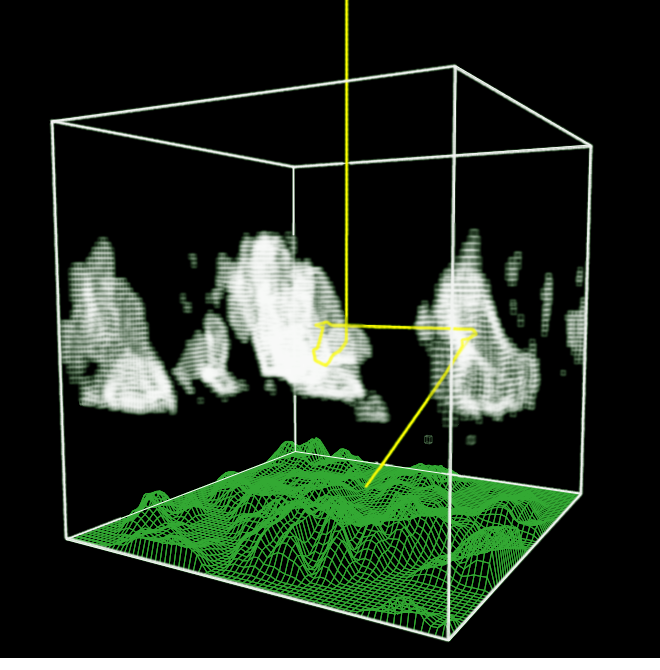
\includegraphics[width=0.7\textwidth]{figs/mystic2.png}\\

  \vfill
  
  % Bottom of the page
  {\large \today}
  
\end{center}

\end{titlepage}
 

%--- Create an empty page
%
\newpage
\thispagestyle{empty}
\rule{0pt}{10pt}
\newpage

\pagenumbering{roman}
\tableofcontents

\cleardoublepage
\pagenumbering{arabic}

%--- Introduction / Preface
\chapter{Preface}
\label{sec:intro}

%\section{A brief overview of libRadtran}

{\sl libRadtran} is a library of radiative transfer routines and
programs.  The central program of the {\sl libRadtran} package is the
radiative transfer tool {\sl uvspec}.  {\sl uvspec} was originally
designed to calculate spectral irradiance and actinic flux in the
ultraviolet and visible parts of the spectrum \citep{kylling92a} where
the name stems from. Over the years, {\sl uvspec} has undergone
numerous extensions and improvements. {\sl uvspec} now includes the
full solar and thermal spectrum, currently from 120~nm to
100~$\mu$m. It has been designed as a user-friendly and versatile tool
which provides a variety of options to setup and modify an atmosphere
with molecules, aerosol particles, water and ice clouds, and a surface
as lower boundary. One of the unique features of {\sl uvspec} is that
it includes not only one but a selection of about ten different
radiative transfer equation solvers, fully transparent to the user,
including the widely-used DISORT code by \citet{Stamnes1988c} and its
C-code version \citep{buras2011b}, a fast two-stream code
\citep{Kylling1995}, a polarization-dependent code polRadtran
\citep{Evans1991}, and the fully three-dimensional Monte
Carlo code for the physically correct tracing of photons in cloudy
atmospheres, MYSTIC \citep{mayer2009, emde2007, emde2010, buras2011a,
emde2011}. MYSTIC optionally allows to consider polarization and fully
spherical geometry. Please note that the public release includes only a
1D version of MYSTIC.

{\sl libRadtran} also provides related utilities, like e.g. a Mie program 
({\sl mie}), some utilities for the calculation of the position of the 
sun ({\sl zenith}, {\sl noon}, {\sl sza2time}), a few tools for 
interpolation, convolution, and integration ({\sl spline}, {\sl conv}, 
{\sl integrate}), and several other small tools for setting up
{\sl uvspec} input and postprocessing {\sl uvspec} output. 

Further general information about {\sl libRadtran} including examples
of use may be found in the
reference publication \citep{mayer2005}. 

It is expected that the reader is familiar with radiative transfer
terminology. In addition, a variety of techniques and
parameterizations from various sources are used. For more information
about the usefulness and applicability of these methods in a specific
context, the user is referred to the referenced literature.

{\sl Please note that this document is by no means complete. It is
under rapid development and major changes will take place.} 


\section*{Acknowledgements}

Many people have already contributed to {\sl libRadtran}'s
development. In addition to Bernhard Mayer (\email{bernhard.mayer (at)
  dlr.de}), Arve Kylling (\email{arve.kylling (at) gmail.com}), Claudia Emde
(\email{claudia.emde (at) lmu.de}), Robert Buras
(\email{robert.buras (at) lmu.de}), Josef Gasteiger
(\email{josef.gasteiger (at) lmu.de}), Bettina Richter
(\email{bettina.richter (at) lmu.de}) and Ulrich 
Hamann (\email{hamann (at) knmi.nl}) the following people have
contributed to {\sl libRadtran} or helped out in various other ways
(the list is almost certainly incomplete -- please let us know if we
forgot somebody):

\begin{itemize}
\item The \code{disort} solver was developed by Knut Stamnes, Warren Wiscombe, 
  S.C.~Tsay, and K.~Jayaweera
\item The translation from the FORTRAN version of the DISORT solver to C-code was performed by Timothy E.~Dowling
\item Warren Wiscombe provided the Mie code \code{MIEV0}, and the routines to calculate
  the refractive indices of water and ice, \code{REFWAT} and \code{ICEWAT}.
\item Seiji Kato (\email{kato (at) aerosol.larc.nasa.gov}) provided the 
  correlated-k tables described in Kato et al. (1999).
\item Tom Charlock (\email{t.p.charlock (at) larc.nasa.gov}), Quiang Fu 
  (\email{qfu (at) atm.dal.ca}), 
  and Fred Rose (\email{f.g.rose (at) larc.nasa.gov}) provided the most recent version 
  of the Fu and Liou code.
\item David Kratz (\email{kratz (at) aquila.larc.nasa.gov}) provided the routines 
  for the simulation of the AVHRR channels described in 
  Kratz (1995).
\item Frank Evans (\email{evans (at) nit.colorado.edu}) provided the
  \code{polradtran} solver.
\item Ola Engelsen provided data and support for different ozone 
absorption cross sections.
\item Albano Gonzales (\email{aglezf (at) ull.es}) included the Yang et
  al. (2000), Key et al. (2002) ice crystal parameterization. 
\item Tables for the radiative properties of ice clouds for different
  particle ``habits'' were obtained from Jeff Key and Ping Yang,
  Yang et al. (2000), Key et al. (2002). In addition, Ping Yang and 
  Heli Wei kindly provided a comprehensive database of particle 
  single scattering properties which we used to derive a consistent 
  set of ice cloud optical properties for the spectral range 0.2 - 100 micron 
  following the detailed description in Key et al. (2002).
  A comprehensive dataset including the full phase matrices has been 
  generated and provided by Hong Gang. 
\item Paul Ricchiazzi (\email{paul (at) icess.ucsb.edu}) and colleagues
  allowed us to include the complete gas absorption parameterization 
  of their model SBDART into {\sl uvspec}.
\item Luca Bugliaro (\email{luca.bugliaro (at) dlr.de}) wrote the analytical 
  TZS solver (thermal, zero scattering).
\item Sina Lohmann (\email{sina.lohmann (at) dlr.de}) reduced the ``overhead time''
  for reading the Kato et al. tables dramatically which resulted in 
  a speedup of a factor of 2 in a twostr solar irradiance calculation.
\item Detailed ice cloud properties were provided by Bryan Baum
  (\email{bryan.baum (at) ssec.wisc.edu}). 
\item Yongxiang Hu (\email{yongxiang.hu-1 (at) nasa.gov}) provided the delta-fit 
  program used to calculate the Legendre coefficients for \code{ic\_properties baum\_hufit}.
\item UCAR/Unidata for providing the \emph{netCDF} library.
\item Many unnamed users helped to improve the code by identifying 
  or fixing bugs in the code. 
\end{itemize}





%--- Radiative transfer theory
\chapter{Radiative transfer theory}
\label{chap:rttheory}

\section{Overview}

Radiative transfer in planetary atmospheres is a complex problem. The
best tool for the solution may vary depending on the problem.
The {\sl libRadtran} package contains numerous tools that handle
various aspects of atmospheric radiative transfer. The main tools
will be presented later in chapter~\ref{chap:rt}. To give the
user a background for the problem to be solved, the theory behind will
briefly be presented below. The radiative transfer
equation is presented first, and solution methods and approximations are 
outlined afterwards. 

The number of equations in this chapter may be intimidating
even for the brave-hearted. If you just want to get things done and
wonder if the {\sl libRadtran} package includes tools that may be used
for your problem, jump directly to chapter~\ref{chap:rt}. Another good
starting point is to try the examples available through the Graphical
User Interface to the \code{uvspec} tool.


\section{The radiative transfer equation}
Quite generally, the distribution of photons in a dilute gas may be
described by the Boltzmann equation\footnote{For a derivation of the
  Boltzmann equation see a textbook on statistical mechanics, for
  example \citet{Reif1965}. Also note that the Boltzmann equation is
  not a fundamental equation. For a derivation of the radiative
  transfer equation from the Maxwell equations see
  \citet{Mishchenko2002}.} 
\begin{eqnarray}
  {\frac{\partial f}{\partial t}} + \nabla_{{\bf r}}({\bf v}\; f ) +
  \nabla_{{\bf p}}({\bf F} \;f ) = Q({\bf r},\hat{n}, \nu, t).
  \label{eq:Boltzmann}
\end{eqnarray}
Here, the photon distribution function $f({\bf r},\hat{n}, \nu,  t)$ 
varies with location (${\bf r}$), direction of propagation
($\hat{n}$), frequency ($\nu$) and time ($t$). It is defined such that
\begin{eqnarray}
f({\bf r},\hat{n}, \nu, t)\;c\; \hat{n}\cdot d{\bf S}\;d\Omega\; d\nu\; dt
  \label{eq:photon_distribution}
\end{eqnarray}
represents the number of photons with frequency between $\nu$ and $\nu+d\nu$
crossing a surface element $d{\bf S}$ in direction $\hat{n}$ into
solid angle $d\Omega$ in time $dt$ (Stamnes 1986). 
The units of $f({\bf r},\hat{n}, \nu, t)$ are $cm^{-3}\; sr^{-1}\; Hz^{-1}$
and $c$ is the speed of light.
Furthermore, $\nabla_{{\bf r}}$ and $\nabla_{{\bf p}}$ are the divergence
operators in configuration and momentum space, respectively. The 
photons may be subject to an external force ${\bf F}({\bf r},\hat{n}, \nu, t)$
and there may be sources and sinks of photons due to collisions and/or
`true' production and loss, which are represented by 
$Q({\bf r},\hat{n}, \nu, t)$. 

In the absence of relativistic effects ${\bf F}=0$, and the photons propagate 
in straight lines with velocity ${\bf v}=c\;\hat{n}$ between
collisions. Using the relation  
\begin{eqnarray}
\nabla_{{\bf r}}({\bf v}\; f ) = f\;\nabla_{{\bf r}}{\bf v} +
{\bf v}\cdot \nabla f  = {\bf v}\cdot \nabla f,
\end{eqnarray}
where {\bf r} and {\bf v} are independent variables,
Eq.~\ref{eq:Boltzmann} may be written as  
\begin{eqnarray}
  {\partial f \over \partial t} + c\;( \hat{n}\cdot \nabla)\; f
  = Q({\bf r},\hat{n}, \nu, t)
\label{eq:Boltzmann_simpler}
\end{eqnarray}
where the ${\bf r}$ subscript on the gradient operator $\nabla$  has
been omitted. 

The differential energy associated with the photon distribution is
\begin{eqnarray}
dE = c\; h\nu\; f\; \hat{n}\cdot d{\bf S} \;d\Omega\; d\nu \; dt.
  \label{eq:diff_energy}
\end{eqnarray}
The specific intensity of photons
$I({\bf r},\hat{n}, \nu, t)$ is defined such that
($\hat{n}\cdot d{\bf S} = \cos \theta \;dS$)
\begin{eqnarray}
dE = I({\bf r},\hat{n}, \nu, t)\; dS \;\cos\theta\; d\Omega\; d\nu \; dt,
  \label{eq2.5}
\end{eqnarray}
which  gives
\begin{eqnarray}
I({\bf r},\hat{n}, \nu, t) = c\; h\nu \;f({\bf r},\hat{n}, \nu, t).
  \label{eq2.6}
\end{eqnarray}
In a steady state situation Eq.~\ref{eq:Boltzmann_simpler} may then be
written as
\begin{eqnarray}
  ( \hat{n}\cdot \nabla)\;I({\bf r},\hat{n}, \nu)  
     = h\nu \;Q({\bf r},\hat{n}, \nu). 
  \label{eq:Boltzmann_rte}
\end{eqnarray}
Eq.~\ref{eq:Boltzmann_rte} may be interpreted as the radiative
transfer equation in a general geometry. However, as long as the
source term $Q({\bf r},\hat{n}, \nu)$ is not specified it is of little
use. First, however, the two most common geometries for radiative
transfer in planetary atmospheres will be described.

\subsection{The streaming term}
The streaming term $\hat{n}\cdot \nabla$ defines the geometry. In
planetary atmospheres the cartesian and spherical geometries are
most common. In cartesian geometry the plane-parallel approximation is
often used while in spherical geometry the pseudo-spherical and
spherical shell approximations are popular.
\subsubsection{Cartesian geometry - plane-parallel atmosphere}
In a Cartesian coordinate system the streaming term may be written
\citep{Rottmann1991,Kuo1996}
\begin{eqnarray}
   \hat{n}\cdot \nabla &=& n_x \frac{\partial}{\partial x} + n_y
   \frac{\partial}{\partial y} + n_z \frac{\partial}{\partial
     z}\nonumber \\ &=&
   \cos\phi\sqrt{1-\mu^2}\frac{\partial}{\partial x} +
   \sin\phi\sqrt{1-\mu^2}\frac{\partial}{\partial y} +
   \mu \frac{\partial}{\partial z},
  \label{eq:CartesianStreamingTerm}
\end{eqnarray}
where $(n_x, n_y, n_z)$ are the components of the unit vector,
$\mu=\cos\theta$ and $\phi$ is the azimuth angle.

In a plane-parallel geometry (Flat Earth approximation) the atmosphere
is divided into parallel layers of infinite extensions in the $x$- and
$y$-directions. This implies that there are no variation in the $x$- and
$y$-directions. Hence, for this approximation the streaming term becomes
\begin{eqnarray}
   \hat{n}\cdot \nabla =  \mu \frac{\partial}{\partial z}.
  \label{eq:PlaneParallelStreamingTerm}
\end{eqnarray}
This approximation is used by numerous radiative transfer solvers,
including the much used DISORT solver \citep{Stamnes1988c}.

\subsubsection{Spherical geometry - pseudo-spherical atmosphere}
In spherical geometry the streaming term becomes\footnote{A derivation
is provided in Appendix~O of \citet{Thomas1999}. The appendix is
available from http://odin.mat.stevens-tech.edu/rttext/.} 
\begin{eqnarray}
   \hat{n}\cdot{\bf\nabla} &=& 
\mu\frac{\partial}{\partial r} + 
\frac{1-\mu^{2}}{r}\frac{\partial}{\partial \mu}  \nonumber \\
&&\!\!\!\!\!\!\!\!\!\!\!\!\!\!\!\!\!\!\!\!\!\!\!\!\!\!\!
+ \frac{\sqrt{1-\mu^{2}}\sqrt{1-{\mu_{0}}^{2}}}{r}\left[
\cos(\phi-\phi_{0})\frac{\partial}{\partial \mu_{0}} +
\frac{\mu_{0}}{1-\mu_{0}^{2}}\sin(\phi-\phi_{0})
\frac{\partial}{\partial (\phi-\phi_{0})} 
\right].
  \label{eq:SphericalStreamingTerm}
\end{eqnarray}

In a spherically symmetric (=spherical shell) atmosphere the streaming term reduces to
\begin{eqnarray}
   \hat{n}\cdot{\bf\nabla} &=& 
\mu\frac{\partial}{\partial r} + 
\frac{1-\mu^{2}}{r}\frac{\partial}{\partial \mu}.
  \label{eq:SphericalSymmetricStreamingTerm}
\end{eqnarray}
\citet{Dahlback1991} has shown that for mean intensities it is
sufficient to include only the first term in
Eq.~\ref{eq:SphericalSymmetricStreamingTerm} for solar zenith angles
up to 90$^{\circ}$. Thus, 
\begin{eqnarray}
   \hat{n}\cdot{\bf\nabla} &=& 
\mu\frac{\partial}{\partial r}.
  \label{eq:PseudoSphericalSymmetricStreamingTerm}
\end{eqnarray}
For this to hold the direct beam must be calculated in spherical
geometry. This is the so-called pseudo-spherical approximation. It
may work well for irradiances, mean intensities and nadir and zenith
radiances. For irradiances in off-zenith and off-nadir directions it
must be shown the angle derivatives are indeed negligible. This is
rarely done in practice.

\subsection{The source term}
The source term on the right hand side of Eq.~\ref{eq:Boltzmann_rte}
includes all losses and gains of radiation in the direction and
frequency of interest. For photons in a planetary atmosphere the
source term may be written as\footnote{For a derivation of the
  individual terms see e.g. \citet{chand60}.}
\begin{eqnarray}
h\nu\;Q( r,\hat{n}, \nu) &=& h\nu\;Q(r, \theta, \phi, \nu)
= -\beta^{ext}(r, \nu)\;
I(r,\theta, \phi, \nu)
\nonumber\\ &&
+\frac{1}{4\pi}\int_{0}^{\infty}\beta^{sca}(r,\nu,\nu')\int_{0}^{2\pi}d\phi '\int_{0}^{\pi}d\theta '
p(r,\theta, \phi; \theta', \phi') 
I( r,\theta ', \phi ', \nu') d\nu'
\nonumber\\ &&
+\beta^{abs}(r, \nu)\;B[T(r)].
  \label{eq:GeneralSource}
\end{eqnarray}
The first term represents loss of radiation due to absorption and
scattering (=extinction)
out of the photon beam. The second term (multiple scattering term) describes the
number of photons scattered into the beam from all other directions
and frequencies, finally, the third term gives the amount of thermal
radiation emitted in the frequency range of interest. 

The lower part of the Earth's atmosphere, may to a good approximation,
be assumed to be in local thermodynamic equilibrium
\footnote{
The hypothesis of local thermodynamic equilibrium (LTE) makes the
assumption that all thermodynamic properties of the medium are the same as
their thermodynamic equilibrium (T.E.) values at the local $T$ and density.
Only the radiation field is allowed to depart from its T.E. value of
$B[T(r)]$ and is obtained from a solution of the transfer equation. Such
an approach is manifestly {\it internally inconsistent}. $\ldots$ 
`However, if the medium is subject  only to {\it small} gradients over the
mean free path a photon can travel before it is destroyed and 
thermalized by a collisional process, then the LTE approach is valid.'
(adapted from \citet[p. 26]{Mihalas1978})}.
Thus, the
emitted radiation is proportional to the Planck function, $B[T(r)]$,
integrated over the frequency or wavelength region of interest.
Furthermore, by Kirchhoff's law the emissivity coefficient $\beta^{emi}$
is equal to the absorption coefficient $\beta^{abs}$.

The absorption, scattering and extinction coefficients are defined as
\citep{Stamnes1986b}
\begin{eqnarray}
\beta^{abs}(r, \nu)=\sum_{i}\beta^{abs}_{i}(r, \nu), &&
\beta^{abs}_{i}(r, \nu)=n_{i}(r) \sigma_{i}^{abs}(\nu)
\label{eq:abs}
\\
\beta^{sca}(r, \nu)=\sum_{i}\beta^{sca}_{i}(r, \nu), &&
\beta^{sca}_{i}(r, \nu)=n_{i}(r) \sigma_{i}^{sca}(\nu)
\label{eq:sca}
\end{eqnarray}
\begin{eqnarray}
\beta^{ext}(r, \nu)=\beta^{abs}(r, \nu)+\beta^{sca}(r, \nu)
\nonumber
\end{eqnarray}
where $n_{i}(r)$ is the density of the atmospheric molecule species $i$ and 
$\sigma_{i}^{abs}(\nu)$ and $\sigma_{i}^{sca}(\nu)$  are the
corresponding absorption and scattering cross sections. The phase function
is defined as
\begin{eqnarray}
p(r, \theta, \phi; \theta ', \phi ', \nu)=
\frac{\sum_{i}\beta_{i}^{sca}(r, \nu)
p_{i}(\theta, \phi; \theta ', \phi ', \nu)}
{\sum_{i}\beta_{i}^{sca}(r, \nu)}
\nonumber
\end{eqnarray}
where the phase function for each species 
\begin{eqnarray}
p_{i}(\theta, \phi; \theta ', \phi ', \nu)=
p_{i}(\cos\Theta, \nu)=
\frac{\sigma_{i}^{sca}(\nu, \cos\Theta)}
{\int_{4\pi}d\Omega\;\sigma_{i}^{sca}(\nu, \cos\Theta)}
\nonumber
\end{eqnarray}
and the scattering angle $\Theta$ is related to the local polar and 
azimuth angles through
\begin{eqnarray}
\cos\Theta = \cos\theta\;\cos\theta ' + \sin\theta\;\sin\theta '\;
\cos(\phi-\phi ').
\nonumber
\end{eqnarray}
The temperature profile, the densities and absorption and scattering 
cross sections are all needed to solve the radiative transfer equation.
Temperatures and densities may readily be obtained from measurements
or atmospheric models. Cross sections are taken from
measurements, from theoretical models or a combination of both.

\subsection{The radiative transfer equation in 1D}
In plane-parallel geometry the monochromatic\footnote{Frequency
  redistribution is required if Raman scattering is included in the
  calculation. For many applications Raman scattering is negligible
  and the photons are assumed not to change frequency. They are
  monochromatic. Thus, all frequency dependence have been suppressed
  in Eq.~\ref{eq:RTE_1D}.}
radiative transfer
equation~\ref{eq:Boltzmann_rte} is written by combining
Eq.~\ref{eq:PlaneParallelStreamingTerm} and
Eq.~\ref{eq:GeneralSource}
\begin{eqnarray}
 - \mu {dI(z,\mu,\phi) \over \beta^{ext}dz}&=& I(z,\mu,\phi) \nonumber\\
 && - {\omega(z) \over 4\pi } \int^{2\pi}_{0}d\phi' \int^{1}_{-1}d\mu'
   p(z,\mu,\phi;\mu',\phi')I(z,\mu',\phi') \nonumber\\
& &-(1-\omega(z))B[T(z)]
  \label{eq:RTE_1D}
\end{eqnarray}
where the single scattering albedo 
\begin{eqnarray}
\omega(z)=\omega(z,\nu)=
\frac{\beta_{i}^{sca}(z, \nu)}{\beta_{i}^{ext}(z, \nu)}=
\frac{\beta_{i}^{sca}(z, \nu)}{\beta_{i}^{abs}(z, \nu)+\beta_{i}^{sca}(z, \nu)}.
\nonumber
\end{eqnarray}
Formally the pseudo-spherical radiative transfer equation is similar
to Eq.~\ref{eq:RTE_1D}, but with $z$ replaced by $r$.



\subsection{Polarization - scalar versus vector}
The intensity or radiance $I$, solved for in the above equations have
a magnitude, a direction and a wavelength. In addition to this light
also possesses a property called polarization. When assuming randomly
oriented particles the radiative transfer equation formally does not
change when including polarization. However, the scalar radiance $I$
is replaced with the vector quantity ${\bf I}$
\begin{eqnarray}
{\bf I} = (I, Q, U, V),
\end{eqnarray}
where $I$, $Q$, $U$ and $V$ are the so-called Stokes parameters (see
e.g. \citet{bohren1998}). Furthermore, the phase function $p(r,\theta,
\phi; \theta', \phi')$ is replaced by the $4\times 4$ phase matrix ${\bf
  P}(r,\theta, \phi; \theta', \phi')$, and if thermal radiation is under
consideration the Stokes emission vector must also be accounted for.

The degree of polarization $p$ is defined as
\begin{equation}
  \label{eq:polarization:pol_degree}
  p = \frac{\sqrt{Q^2 + U^2 + V^2}}{I}.
\end{equation}
For completely polarized radiation, $Q^2 + U^2 + V^2 = I^2$, thus $p =
1$, and for unpolarized radiation, $Q = U = V = 0$, thus $p = 0$.

In addition to the degree of polarization, $p$, the degree of linear
polarization is defined as
\begin{equation}
  \label{eq:polarization:p_lin}
 p_{lin} = \frac{\sqrt{Q^2 + U^2}}{I},
\end{equation}
and the the degree of circular polarization is defined as
\begin{equation}
  \label{eq:polarization:p_circ}
 p_{circ} = \frac{V}{I}. 
\end{equation}
Polarization is often ignored in radiative transfer calculations both
due to the complexity involved in the solution of the RTE including
polarization and the higher demand on computer resources by these
solution methods. Also, for many applications polarization may be
ignored. If you are concerned about your specific application,
\code{uvspec} makes it easy to change solvers and thus readily allows 
comparisons to be made between scalar and vector calculations.


\section{General solution considerations}
A multitude of methods exist to solve the radiative transfer
equation~\ref{eq:Boltzmann_rte}. Most methods have some commonalities
and they are briefly described below.

\subsection{Direct beam/diffuse radiation splitting}
The integro-differential radiative transfer
equation~\ref{eq:Boltzmann_rte} gives the radiance field when solved
with  appropriate boundary conditions, that is, the 
radiation incident at the bottom and the top of the atmosphere. At the 
bottom of the atmosphere the Earth partly reflects radiation and also
emits radiation as a quasi-black-body. At the top of the atmosphere
($z=z_{{\text{toa}}}$) a parallel beam of  sunlight with magnitude
$I^{0}$ in the direction $\mu_{0}$ may be present
\begin{eqnarray}
I(z_{{\text toa}},\mu)= I^{0} \delta(\mu-\mu_{0}),
  \label{eq:Boundary_toa}
\end{eqnarray}
where $\delta(\mu-\mu_{0})$ is the Dirac delta-function. It is akward
to use a delta function for a boundary condition. However, a
homogeneous differential equation with inhomogeneous boundary conditions
may always be turned into an inhomogeneous differential equation with
homogeneous boundary conditions. Since the  integro-differential
equation~\ref{eq:Boltzmann_rte} is already inhomogeneous, the addition
of another inhomogeneous term does not necessarily complicate the problem.
Hence  the intensity field is written as the sum of the direct
($\text{dir}$) and the scattered ($\text{sca}$)(or diffuse) radiation
\begin{eqnarray}
I(z,\mu, \phi)=I^{\text{dir}}(z,\mu_0, \phi_0)+I^{\text{sca}}(z,\mu, \phi),
\label{eq:DirectDiffuse}
\end{eqnarray}
where $\mu_0$ and $\phi_0$ are the solar zenith and azimuth angles
respectively. Inserting Eq.~\ref{eq:DirectDiffuse} into
Eq.~\ref{eq:Boltzmann_rte} it is seen that the direct beam satisfies
\begin{eqnarray}
-\mu\frac{dI^{\text{dir}}(z,\mu_0, \phi_0)}{\beta^{ext}dz}=
-\mu\frac{dI^{\text{dir}}(z,\mu_0, \phi_0)}{d\tau}=I^{\text{dir}}(z,\mu_0, \phi_0)
  \label{eq:DirectRTE}
\end{eqnarray}
where the optical depth is defined as $d\tau = \beta^{ext}dz$.
The scattered intensity satisfies in 1D (the $\text{sca}$
superscript is omitted) 
\begin{eqnarray}
 - \mu {dI(\tau,\mu, \phi) \over d\tau}& =& I(\tau,\mu, \phi) 
 \nonumber \\ & & -
  {\omega(r) \over 4\pi } \int^{2\pi}_{0}d\phi' \int^{1}_{-1}d\mu'
   p(\tau,\mu, \phi;\mu', \phi')I(\tau,\mu', \phi)
 \nonumber \\ & & 
   -(1-\omega(\tau))B[T(\tau)] 
\nonumber \\
& &    -\frac{\omega(\tau)I^{0}}{4\pi}p(\tau,\mu, \phi;\mu_{0}, \phi_0 )e^{-\tau/\mu_{0}}.
  \label{eq:DiffuseRTE}
\end{eqnarray}
Solution of Eq.~\ref{eq:DirectRTE} for the direct beam yields the 
Beer-Lambert-Bouguer law
\begin{eqnarray}
I^{dir}(\tau,\mu_0)=I^{0}\;e^{-\tau/\mu_{0}}.
  \label{eq:Beerlaw}
\end{eqnarray}
The popular {\bf disort} solver \citep{Stamnes1988c,stamnes2000}
solves Eqs.~\ref{eq:DirectRTE}-\ref{eq:DiffuseRTE}.

\subsection{Pseudo-spherical approximation}
In the pseudo-spherical approximation the extinction path
$\tau/\mu_{0}$ in Eqs.~\ref{eq:DiffuseRTE} and \ref{eq:Beerlaw} is
replaced by the Chapman function, $ch(r,\mu_{0})$
\citep{Rees1989B,Dahlback1991}
\begin{eqnarray}
ch(r_{0},\mu_{0})=\int_{r_{0}}^{\infty}
              \frac{\beta^{ext}(r,\nu)\;dr}
        {\sqrt{1-\left(\frac{R+r_{0}}{R+r}\right)^{2}
         \left(1-\mu^{2}_{0}\right)}}.
  \label{eq2.24}
\end{eqnarray}
Here $R$ is the radius of the earth and $r_{0}$ the distance above the
earth's surface. The Chapman function describes the extinction
path in a spherical atmosphere.

Thus, in the pseudo-spherical approximation the direct beam is
correctly described by
\begin{eqnarray}
I^{dir}(r,\mu)=I^{0}\;e^{-ch(r,\mu_{0})}
  \label{eq:pseudoBeer}
\end{eqnarray}
and the diffuse radiation is approximated by replacing the
plane-parallel direct beam source in Eq.~\ref{eq:DiffuseRTE} with the
corresponding direct beam source in spherical geometry
\begin{eqnarray}
 - \mu {dI(\tau,\mu, \phi) \over d\tau}& =& I(\tau,\mu, \phi) 
 \nonumber \\ & & -
  {\omega(r) \over 4\pi } \int^{2\pi}_{0}d\phi' \int^{1}_{-1}d\mu'
   p(\tau,\mu, \phi;\mu', \phi')I(\tau,\mu', \phi)
 \nonumber \\ & & 
   -(1-\omega(\tau))B[T(\tau)] 
\nonumber \\
& &    -\frac{\omega(\tau)I^{0}}{4\pi}p(\tau,\mu, \phi;\mu_{0}, \phi_0 )e^{-ch(\tau,\mu_{0})}.
  \label{eq:pseudoDiffuseRTE}
\end{eqnarray}
The {\bf sdisort} solver included in the libRadtran software package
\citep{mayer2005} solves
Eqs.~\ref{eq:pseudoBeer}-\ref{eq:pseudoDiffuseRTE}. 

\subsection{Boundary conditions}
The diffuse radiative transfer Eq.~\ref{eq:DiffuseRTE} is solved
subject to boundary conditions at the top and bottom of the
atmosphere. At the top boundary there is no incident diffuse
intensity\footnote{The DISORT type RTE-solvers, {\bf disort 1.3}, {\bf
    disort 2.0}, {\bf sdisort} and {\bf twostr}, may include a diffuse
  radiation source at the top boundary. This may be of interest when
  for example modelling the aurora.}
($\mu \ge 0$) 
\begin{eqnarray}
I(\tau=0, -\mu, \phi )=0.
  \label{eq:TopBoundary}
\end{eqnarray}
The bottom boundary condition may quite generally be formulated in
terms of a bidirectional reflectivity, $\rho(\mu,\phi;-\mu',\phi')$,
and directional emissivity, $\epsilon(\mu)$,
\begin{eqnarray}
  I(\tau=\tau_g, \mu, \phi ) &=& \epsilon(\mu) B[T(\tau_{g})]
  + \frac{1}{\pi} \mu_0 I_0 e^{-\tau_g/\mu_{0}}
  \rho(\mu,\phi;-\mu',\phi') \nonumber \\
  && +\frac{1}{\pi} \int_0^{2\pi} d\phi' \int_0^1
  \rho(\mu,\phi;-\mu',\phi')  I(\tau,-\mu', \phi') \mu' d\mu' ,
  \label{eq:BottomBoundary}
\end{eqnarray}
where $T(\tau_{g})$ is the temperature of the bottom boundary, here
the Earth's surface.

In the case of a Lambertian reflecting bottom boundary with albedo
$\rho(\mu,\phi;-\mu',\phi')=A$,
Eq.~\ref{eq:BottomBoundary} simplifies to
\begin{eqnarray}
\pi I(\tau_{L}, \mu )&=& \pi\;\epsilon \;B[T(\tau_{g})]+
\mu_{0}\;A\;I^{0}e^{-\tau_{g}/\mu_{0})} \nonumber \\
&&+ 2\pi\; A \int_0^{2\pi}
d\phi' \int_{0}^{1} \mu I(\tau_{L},-\mu, \phi) d\mu.
  \label{eq:BottomBoundarySimple}
\end{eqnarray}
The albedo, $A$, gives the fraction of reflected light under the
assumption that the surface reflects radiation isotropically (Lambert
reflector). The emissivity $\epsilon = 1-A$, by Kirchhoff's law.
In both Eqs.~\ref{eq:BottomBoundary} and
\ref{eq:BottomBoundarySimple} the first term on the right hand side is
the thermal radiation emitted by 
the surface. The second term is due to reflection of the direct beam
that has penetrated through the whole atmosphere and the last term 
is reflection of downward diffuse radiation

\subsection{Separation of the azimuthal $\Phi$-dependence, Fourier decomposition}
For scattering processes in the atmosphere the scattering phase
function depends only on the angle $\Theta$ between the incident and
scattered beams. This may be used to seperate out the
$\Phi$-dependence in Eqs.~\ref{eq:DiffuseRTE} and
\ref{eq:pseudoDiffuseRTE} as follows. The phase function is first
expanded as a series of Legendre polynomials
\begin{eqnarray}
  p(\tau,\mu, \phi;\mu', \phi') = p(\tau,\Phi) = \sum_{l=0}^{2M-1}
  (2l+1) g_l(\tau) p_l(\cos\Phi)
  \label{eq:PhaseFunction}
\end{eqnarray}
where the phase function moments $g_l$ are given by
\begin{eqnarray}
  g_l(\tau) = {1 \over 2} \int_{-1}^{+1} p_l(\cos\Phi)p(\tau,\Phi)d(\cos\Phi).
  \label{eq:PhaseFunctionMoment}
\end{eqnarray}
The $g_1$ term is called the ``asymmetry factor'', and $g_0=1$ due to
normalization of the phase function. Applying the addition theorem for
spherical harmonics to Eq.~\ref{eq:PhaseFunction} gives
\begin{eqnarray}
p(\tau,\Phi) = \sum_{l=0}^{2M-1}  (2l+1) g_l(\tau)\left\{
    p_l(\mu) p_l(\mu') + 2\sum_{m=1}^{l} \Lambda_l^m(\mu)
    \Lambda_l^m(\mu') \cos m(\phi-\phi') \right\}\nonumber \\
  \label{eq:PhaseFunctionSphericalHarmonics}
\end{eqnarray}
where the normalized associated Legendre polynomials are defined as
\begin{eqnarray}
  \Lambda_l^m(\mu) = \sqrt{\frac{(l-m)!}{(l+m)!}} P_l^m(\mu),
  \label{eq:NormalizedAssociatedLegendrePolynomial}
\end{eqnarray}
and $P_l^m(\mu)$ are the standard Legendre polynomials. The cosine
dependence of the phase function,
Eq.~\ref{eq:PhaseFunctionSphericalHarmonics}, suggests that cosine
expansion of the intensity may be fruitful. Expanding the intensity as
a cosine Fourier series:
\begin{eqnarray}
  I(\tau,\mu,\phi) = \sum_{l=0}^{2M-1} I^m(\tau,\mu)  \cos m(\phi_0-\phi)
  \label{eq:CosineExpansion}
\end{eqnarray}
and inserting into Eqs.~\ref{eq:DiffuseRTE} and
\ref{eq:pseudoDiffuseRTE} gives $2M$ independent integro-differential
equation (only the plane-parallel version is shown here)
\begin{eqnarray}
 - \mu {dI^m(\tau,\mu) \over d\tau}& =& I^m(\tau,\mu) 
 \nonumber \\ & & -
  {\omega(r) \over 2 } \int^{1}_{-1}d\mu'
   \sum_{l=m}^{2M-1} (2l+1) g_l(\tau) \Lambda_l^m(\mu) \Lambda_l^m(\mu') I^m(\tau,\mu')
 \nonumber \\ & & 
   -\delta_{m0}(1-\omega(\tau))B[T(\tau)] 
\nonumber \\
& &    -\frac{\omega(\tau)I^{0}}{4\pi} (2-\delta_{m0}) 
        \sum_{l=m}^{2M-1} (2l+1) g_l(\tau) \Lambda_l^m(\mu) \Lambda_l^m(\mu') e^{-\tau/\mu_{0}}.\nonumber\\
  \label{eq:DiffuseRTEseparated}
\end{eqnarray}
where 
\begin{displaymath}
\delta_{m0} = \left\{ \begin{array}{ll}
      1 & \text{if $m=0$} \\
      0 & \text{if $m\neq 0$} 
      \end{array} \right.
\end{displaymath}



\subsection{Calculated quantities}
Solution of the radiative transfer equation generally yields the
diffuse radiance
\begin{eqnarray}
  I(\tau, \mu, \phi)
  \label{eq:Radiance}
\end{eqnarray}
and the direct radiance
\begin{eqnarray}
  I^{\text dir}(\tau, \mu_0, \phi_0).
  \label{eq:DirectRadiance}
\end{eqnarray}
For the solvers that include polarization the vector quantities of the
above quantities are calculated.
From these quantities the upward, $E^{+}(\tau)$, and downward,
$E^-(\tau)$, fluxes, or irradiances, are calculated
\begin{eqnarray}
E^+(\tau) &=& \int_0^{2\pi} d\phi \int_{0}^{1} \mu I(\tau,\mu, \phi) d\mu 
  \label{eq:UpwardFlux} \\
E^-(\tau) &=& \mu_0 I_0 e^{-\tau/\mu_0} + \int_0^{2\pi} d\phi \int_{0}^{1} \mu I(\tau,-\mu, \phi) d\mu.
  \label{eq:DownwardFlux}
\end{eqnarray}
Furthermore, the mean intensity 
\begin{eqnarray}
  \overline{I}(\tau) &=& \frac{1}{2\pi} \left[ I_0 e^{-\tau/\mu_0} +
 \int_0^{2\pi}d\phi \int_{0}^{1} I(\tau,-\mu, \phi) d\mu + 
 \int_0^{2\pi}d\phi \int_{0}^{1}  I(\tau,\mu, \phi) d\mu \right],\nonumber\\
  \label{eq:MeanIntensity} 
\end{eqnarray}
is related to the actinic flux
\citep{Madronich1987b}, $F$, used for the calculation of photolysis
(or photodissociation) rates
\begin{eqnarray}
  F(\tau) &=& 4 \pi \overline{I}(\tau).
  \label{eq:ActinicFlux} 
\end{eqnarray}
Finally, heating rates may be calculated from either the flux
differences or the mean intensity.
\begin{eqnarray}
  \frac{\partial T}{\partial t} &=& -\frac{4\pi}{c_p \rho_m}
  \frac{\partial E}{\partial z} =  -\frac{4\pi}{c_p \rho_m}
  (1-w)(\overline{I}-B)\frac{\partial \tau}{\partial z}.
  \label{eq:HeatingRate} 
\end{eqnarray}
Note that the partial derivative of $\tau$ with respect to $z$ is needed
since optical properties and $\overline{I}$ are calculated as functions
of $\tau$.

The various radiative transfer equation solvers included in the
\code{uvspec} tools in the {\sl libRadtran} package, have different
capabilities to calculate the above 
radiative quantities. The user is referred to
section~\ref{sec:RTEsolvers} for an overview of the different
solvers included in the \code{uvspec} program and their respective
capabilities. For a complete description of all solvers with options
section~\ref{sec:uvspec_options} should be consulted. Finally, there
is nothing to complement a thorough understanding of the problem at
hand, the theory behind the chosen solution and a little reading of
the code itself. 

\subsection{Lidar equation}

The lidar equation can be written as (see e.g.~\citet{Weitkamp2005})
%
\begin{equation}
%
\frac{{\rm d}N(r)}{{\rm d}r} =
  \frac{E_0}{E_{\rm phot}} A_{\rm det} \eta \frac{O(r)}{4 \pi r^2}
  p(\cos \pi) \beta^{sca}(r)
  \exp\left(-2\int_0^r dr' \beta^{ext}(r')\right),
%
\label{eq:sslidar}
\end{equation}
%
where $N(r)$ is the number of detected photons, $E_0$ is the energy
per laser pulse, $E_{\rm phot}$ is the energy per photon, $A_{\rm
  det}$ is the detector area, $\eta$ is the detector efficiency,
$O(r)$ is the overlap function, $r$ is the range, and $p(\cos \pi)$ is
the scattering phase function in backward direction. Note that the
nomenclature here is consistent with the libRadtran documentation and
differs from that in most lidar papers and books.

The lidar equation is a solution of the RTE for the special problem of
a lidar signal, and is a single scattering approximation to the real
world. Nevertheless it is applicable for many cases of interest. For
space-borne lidars it should not be used.

Many lidarists are also interested in the lidar ratio, which is
defined as
%
\begin{equation}
%
S(r) = \frac{4 \pi}{p(\cos \pi) \omega(r)}.
%
\label{eq:lidar_ratio}
\end{equation}
%

For the special case of Lambertian surface reflection, the signal is
%
\begin{equation}
%
N_{\rm surf}(r_{\rm surf}) =
  \frac{E_0}{E_{\rm phot}} A_{\rm det} \eta \frac{O(r_{\rm surf})}{4 \pi r_{\rm surf}^2}
  4 a \cos \theta_{\rm refl}
  \exp\left(-2\int_0^{r_{\rm surf}} dr' \beta^{ext}(r')\right),
%
\label{eq:sslidar_surf}
\end{equation}
%
where $r_{\rm surf}$ is the range of the surface, $a$ is the surface
albedo, and $\theta_{\rm refl}$ is the inclination with which the
laser beam hits the surface.

\subsection{Verification of solution methods}
To solve the radiative transfer equation involves complex numerical
procedures that are difficult both to develop and to implement. Great
care must be taken during implementation to assure that the numerical
procedure is stable for any values and combinations of 
the input parameters, i.e. optical depth, single scattering albedo, phase
function and boundary conditions. The testing of new solvers are
typically done by the developers against analytical solutions which
are available for a few special cases. Furthermore, tests and
comparisons are made against other models and measurements. The reader
is referred to the individual papers describing the various solvers
for more information.

The input quantities needed by the solvers are optical depth, single
scattering albedo, phase function and boundary conditions. These are
calculated from atmospheric profiles of molecular density, trace gas
species, water and ice clouds and aerosols. In addition,
the absorption and scattering properties of the various species are
taken from measurements or model calculations. The calculation of the
optical properties are compared against other models and measurements
during code development.




%--- Radiative transfer simulations
\chapter{Radiative transfer simulations - {\sl uvspec}}
\label{chap:rt}

%\section{Overview}
The {\sl uvspec} program calculates the radiation field in the
Earth's atmosphere. Input to the model are the constituents of the
atmosphere including various molecules, aerosols and clouds. The
absorption and scattering properties of these constituents may either
be taken from the algorithms and databases provided with {\sl
  libRadtran} and {\sl uvspec} or be provided by the user. Boundary
conditions are the solar spectrum at the top of the atmosphere and the
reflecting surface at the bottom. Several extraterrestrial solar
spectra are provided with {\sl libRadtran} and various surface models
are also included. 

{\sl uvspec} is structured into the following three
essential parts:  (1) An atmospheric shell 
which converts atmospheric properties like ozone profile, surface
pressure, or cloud microphysical parameters into optical properties
required as input to (2) the radiative transfer equation solver which
calculates radiances, irradiances, actinic fluxes and heating rates
for the given optical properties; and (3) post-processing of the
solver output including multiplication with the extraterrestrial solar
irradiance correction of Earth-Sun distance, convolution with a
slit-function, or integration over wavelength (depending on the choice
of the user). For an overview see Figure~\ref{fig:uvspec_structure}.
\begin{figure}[htbp]
  \centering
  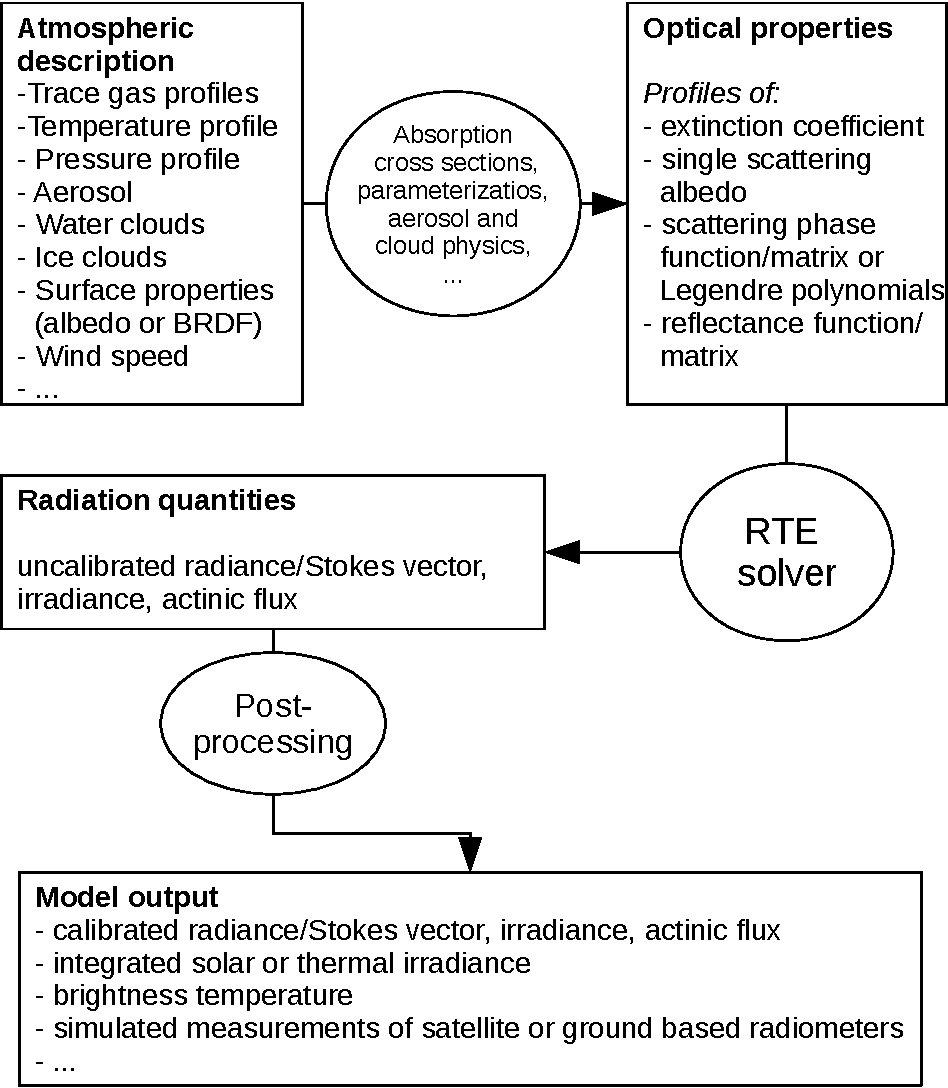
\includegraphics[width=0.9\textwidth]{figs/figure1}
  \caption{Structure of the {\sl uvspec} model}
  \label{fig:uvspec_structure}
\end{figure}


The core of all radiative transfer models is a method to calculate the
radiation field for a given distribution of optical properties by
solving the radiative transfer equation. To solve the radiative
transfer equation discussed in Chapter~\ref{chap:rttheory} 
{\sl uvspec} has the unique feature of giving the user a choice of
various  radiative transfer solvers (table~\ref{tab:rte_solvers}).
This implies that for the radiative transfer problem at hand an
appropriate solver may 
be chosen, e.g. a fast two-stream code to calculate approximate
irradiance or a discrete ordinate code to accurately simulate
radiances, with or without polarization. 
\ifmystic{
  The full 3D radiative 
  transfer equation may be solved by the Monte Carlo solver MYSTIC. Please note
  that the public release includes only a 1D version of MYSTIC.}

Below the basic usage of {\sl uvspec} is described first followed by
a general description of the {\sl uvspec} input file and output file. The
{\sl uvspec} input file may either be generated manually using any
text editor capable of saving files in ASCII (plain text) format, or
it may be generated by the {\sl uvspec} Graphical User Interface
found in the \file{GUI} folder. The input/output file description is 
followed by a brief description of the radiative transfer equation solvers 
available in {\sl uvspec}. Finally several examples of usage of {\sl uvspec} 
are given.

\section{Basic usage}

\subsection{Running {\sl uvspec}}

{\sl uvspec} reads 
from standard input, and outputs to standard output. It is normally
invoked in the following way\footnote{The Graphical User Interface to
{\sl uvspec} provides another convenient way. \index{uvspec@{\sl uvspec} as
a callable function} {\sl uvspec}
may also be called as a function from another C program. See
\file{src/worldloop.c} for an example.}:

\begin{Verbatim}[fontsize=\footnotesize] 
  uvspec < input_file > output_file
\end{Verbatim}
  
\noindent The formats of the input and output files are described
below. Several realistic examples of input files are 
given in section~\ref{sec:examples}.

\noindent {\sl uvspec} may produce a wealth of diagnostic
messages and warnings, depending on your use of \codeidx{verbose} or
\codeidx{quiet}.  Diagnostics, error messages, and warnings are written
to \code{stderr} while the {\sl uvspec} output is written to
\code{stdout}. To make use of this extra information, you may want to
write the standard {\sl uvspec} output to one file and the diagnostic
messages to another. To do so, try \code{(./uvspec < uvspec.inp >
uvspec.out) >\& verbose.txt}. The irradiances and radiances will be
written to \file{uvspec.out} while all diagnostic messages go into
\file{verbose.txt}. This method can also be used to collect
{\sl uvspec} error messages.

{\bf Warning:} Please note the error checking on input variables is
not complete at the moment. Hence, if you provide erroneous input, the
outcome is unpredictable.

\subsection{The {\sl uvspec} input file}

{\sl uvspec}
is controlled in a user-friendly way. The control options are named in
a (hopefully) intuitive way. 

The {\sl uvspec} input file consists of single line entries, each
making up a complete input to {\sl uvspec}. First on the
line comes the option name, followed by one or more parameter
values. The option name and the parameter values are separated by
white space.  Filenames are entered without any surrounding single or
double quotes.  Comments are introduced by a \code{\#}. Blank lines
are ignored. The order of the lines is not important, with one
exception: if the same input option is used more than once, the second
one will usually over-write the first one. Be aware that also options
in another included input file will overwrite options specified
before.


\subsection{How to setup an input file for your problem (checklist)}

There are several steps to consider when setting up an input file for
your specific problem. First of all we strongly recommend that you
read a radiative transfer textbook to become familiar with what is
required for your problem. Below is a short checklist including the
steps you need to consider for each problem:

\begin{enumerate}

\item {\bf Wavelength grid / band parameterization}
 
  By default, libRadtran employs the REPTRAN band parameterization 
  with a spectral resolution of 15~cm$^{-1}$. It allows to calculate
  quantities integrated over narrow spectral bands. You need to
  specify a wavelength range using \codeidx{wavelength}. 
  The wavelengths for which the radiative transfer calculations are performed are
  determined by the parameterization and implicitly consider 
  high-spectral-resolution features of molecular absorption within each band. 
  With \codeidx{wavelength\_grid\_file} pseudo-spectral 
  calculations can be performed, meaning that you can calculate radiation 
  at any wavelength you want, but it is always a weighted mean calculated 
  from radiative transfer calculations at so-called representative 
  wavelengths of the belonging band - if you select the wavelengths too close, 
  you will see the steps in your spectrum. \codeidx{wavelength\_grid\_file} is particularly useful
  if the default resolution is too expensive for your application.
  If you need a higher spectral resolution of the band data use 
  \code{mol\_abs\_param reptran fine/medium}.

  The spectral parameterizations can be switched off with \code{mol\_abs\_param crs}.
  This can be necessary for example for wavelength below 205nm, or 
  if you want to use your own high-spectral resolution atmospheric data.
  In this case, the radiative transfer calculations are performed on
  the grid provided by \codeidx{wavelength\_grid\_file}. 
  Finally, in order to calculate integrated
  shortwave or integrated longwave radiation, please choose one of the
  pre-defined correlated-k distributions, e.g. 
  \code{mol\_abs\_param kato2} or 
  \code{mol\_abs\_param fu} because these are not only much more
  accurate but also much faster than a pseudo-spectral
  calculation. Please read the respective sections in the manual to
  become familiar with the \codeidx{mol\_abs\_param} options.
  
\item {\bf Quantities}
  
  The next point one needs to consider is the desired radiation
  quantity. Per default, {\sl uvspec} provides direct, diffuse downward
  and diffuse upward solar irradiance and actinic flux at the
  surface. Thermal quantities can be calculated with \code{source thermal} 
  \index{source} -
  please note that {\sl uvspec} currently does either solar or thermal,
  but not both at the same time. If both components are needed (e.g. for
  calculations around 3$\mu$m) then {\sl uvspec} needs to be called
  twice. To calculate radiances in addition to the irradiances, simply
  define \code{umu}, \code{phi}, and \code{phi0} (see next section).
  
\item{\bf Geometry}

  Geometry includes the location of the sun which is defined with \codeidx{sza}
  (solar zenith angle) and \codeidx{phi0} (azimuth). The azimuth is only required
  for radiance calculations. Please note that not only the solar zenith
  angle but also the sun-earth-distance change in the course of the year
  which may be considered with \codeidx{day\_of\_year} (alternatively,
  \code{latitude}, \code{longitude}, and \code{time} may be used). The altitude of the
  location may be defined with \codeidx{altitude} which modifies the profiles
  accordingly. Radiation at locations different from the surface may be
  calculated with \codeidx{zout} which gives the sensor altitude above the
  ground. For satellites use \code{zout TOA} (top of atmosphere). For
  radiance calculations define the cosine of the viewing zenith angle
  \codeidx{umu} and the sensor azimuth \codeidx{phi} and don't forget to also specify the
  solar azimuth \code{phi0}. \code{umu>}0 means sensor looking downward (e.g. a
  satellite), \code{umu<}0 means looking upward. \code{phi} = \code{phi0} indicates that the
  sensor looks into the direction of the sun, \code{phi}-\code{phi0} = 180$^\circ$ means that
  the sun is in the back of the sensor.

\item{\bf What do you need to setup the atmosphere?}

  To define an atmosphere, you need at least an \codeidx{atmosphere\_file}
  which usually contains profiles of pressure, temperature, air density,
  and concentrations of ozone, oxygen, water vapour, carbon dioxide, and
  nitrogen dioxide. The set of six standard atmospheres provided with
  libRadtran is usually a good start: \code{midlatitude\_summer},
  \code{midlatitude\_winter}, \code{subarctic\_summer},
  \code{subarctic\_winter}, \code{tropical}, and \code{US-standard}. If
  you don't define anything else, you have an atmosphere with Rayleigh
  scattering and molecular absorption, but neither clouds, nor aerosol.
  
  \begin{enumerate}
  \item {\bf Trace gases?}
    
    Trace gases are already there, as stated above. But sometimes you
    might want to modify the amount. There is a variety of options to do
    that, e.g. \code{mol\_modify O3} which modifies the ozone column, or
    \code{mixing\_ratio CO2}, \dots
    
  \item {\bf Aerosols?}
    
    If you want aerosol, switch it on with \codeidx{aerosol\_default} and
    use either the default aerosol or one of the many \code{aerosol\_}
    options to setup whatever you need.
    
  \item {\bf Clouds?}
    
    {\sl uvspec} allows water and ice clouds. Define them with
    \codeidx{wc\_file} and \codeidx{ic\_file} and use one of the many \code{wc\_}
    or \code{ic\_} options to define what you need. Please note that for
    water and ice clouds you also have a choice of different
    parameterizations, e.g. \code{ic\_properties fu}, \code{yang},
    \code{baum}, \dots - these are used to translate from liquid/ice water
    content and droplet/particle radius to optical properties. You need
    some experience with clouds to define something reasonable. Here are
    two typical choices for a \code{wc\_file 1D}
    \begin{Verbatim}[fontsize=\footnotesize, frame=single] 
      # z[km] LWC[g/m3] Reff[um]
          2        0        0 
          1      0.1       10
    \end{Verbatim} 
    and an \code{ic\_file 1D}
    \begin{Verbatim}[fontsize=\footnotesize, frame=single] 
      # z[km] IWC[g/m3] Reff[um]
          10         0       0 
           9     0.015      20
    \end{Verbatim}
    The first is a water cloud with effective droplet radius of 10$\mu$m
    between 1 and 2~km, and an optical thickness of around 15; the second
    is an ice cloud with effective particle radius 20$\mu$m between 9 and
    10~km and an optical thickness of about 1.
    
  \item {\bf Surface properties?}
    
    Per default, the surface albedo is zero - the surface absorbs all
    radiation. Define your own monochromatic albedo, a spectral
    \codeidx{albedo\_file} or a BRDF, e.g. for a water surface which is mainly
    determined by the wind speed \codeidx{brdf\_cam u10}.
    
  \end{enumerate}
  
\item {\bf Choice of the radiative transfer equation (RTE) solver}
  
  \index{rte\_solver}
  The RTE-solver is the engine, or heart, in any radiative transfer
  code. All RTE-solvers involve some approximations to the radiative
  transfer equations, or the solution has some uncertainties due to
  the computational demands of the solution method. The choice of
  RTE-solver depends on your problem. For example, if your
  calculations involves a low sun you should not use a plane-parallel
  solver, but one which somehow accounts for the spherical shape of
  the Earth. You may choose between many RTE-solvers in
  {\sl uvspec}. The default solution method to the radiative transfer
  is the discrete ordinate solver \code{disort} which is the method
  of choice for most applications. There are other solvers like
  \code{rte\_solver twostr} (faster but less accurate),
  \code{rte\_solver polradtran} (polarization-dependent solver), or
  \code{rte\_solver sdisort} (pseudo-spherical)\ifmystic{, or \code{rte\_solver
      mystic} (three-dimensional, polarization-dependent solver,
    spherical geometry)}. Even
  lidars can be simulated using \code{rte\_solver sslidar}.
  
\item {\bf Postprocessing}
  
  The spectral grid of the output is defined by the extraterrestrial
  spectrum, which can be modified using \codeidx{source solar file}.
  If you want spectrally integrated results, use either \code{output\_process integrate} 
  for \code{mol\_abs\_param lowtran} and \code{mol\_abs\_param reptran}, 
  or \code{output\_process sum} for \code{mol\_abs\_param kato2}.
  Check also other options like \codeidx{filter\_function\_file}, \codeidx{output\_quantity brightness},
  etc. Instead of calibrated spectral quantities you might also want
  \codeidx{output\_quantity transmittance} or \codeidx{output\_quantity reflectivity}.
  
\item {\bf Check your input}
  
  Last but not least, make always sure that {\sl uvspec} actually
  does what you want it to do! A good way to do that is to use
  \codeidx{verbose} which produces a lot of output. To reduce the amount,
  it is a good idea to do only a monochromatic calculation. Close to the
  end of the verbose output you will find profiles of the optical
  properties (optical thickness, asymmetry parameter, single scattering
  albedo) which give you a pretty good idea, e.g. if the clouds which you
  defined are already there, where the aerosol is, etc. As a general
  rule, never trust your input, but always check, play around, and
  improve. For if thou thinkest it cannot happen to me and why bother to
  use the verbose option, the gods shall surely punish thee for thy
  arrogance!
  
\end{enumerate}

\subsection{How to translate old input files?}
\label{sec:translate}

Since {\sl libRadtran} version 1.8 input option names have changed.
In the directory src\_py/ you will find a program translate.py 
to translate old style input files to new style input files.

To translate your input file use the following command:
\fcode{
python translate.py filename
}

To save the output into a new filename use:
\fcode{
python translate.py filename -\,-new\_filename=new\_inputname
}

To overwrite your old input file use:
\fcode{
python translate.py filename -\,-new\_filename=filename -\,-force
}


\subsection{Output from {\sl uvspec}}
\label{sec:model_output}

The {\sl uvspec} output depends on the radiative transfer solver. The output
formats are described in the following. The meaning of the symbols is
described in Table~\ref{tab:symbols}. The output may be user
controlled to some degree using the option \code{output\_user}.

\subsubsection{disort, sdisort and spsdisort}
For the disort, sdisort and spsdisort solvers {\sl uvspec} outputs
one block of data to 
standard output (stdout) for each wavelength. 

If \code{umu} is not specified the format of the block
is
\begin{Verbatim}[fontsize=\footnotesize, frame=single]  
lambda edir edn eup uavgdir uavgdn uavgup
\end{Verbatim}

If \code{umu} is specified the format of the block is
\begin{Verbatim}[fontsize=\footnotesize, frame=single]  
lambda edir edn eup uavgdir uavgdn uavgup umu(0)
u0u(umu(0)) umu(1) u0u(umu(1)) .  .  .  .
\end{Verbatim}

If both \code{umu} and \code{phi} are specified the output
format of each block is
\begin{Verbatim}[fontsize=\footnotesize, frame=single, samepage=true]   
lambda edir edn eup uavgdir uavgdn uavgup 
                           phi(0)    ...    phi(m) 
umu(0) u0u(umu(0)) uu(umu(0),phi(0)) ... uu(umu(0),phi(m))
umu(1) u0u(umu(1)) uu(umu(1),phi(0)) ... uu(umu(1),phi(m)) 
  .         .           .                        .
  .         .           .                        .
umu(n) u0u(umu(n)) uu(umu(n),phi(0)) ... uu(umu(n),phi(m))
\end{Verbatim}
and so on for each wavelength.


\subsubsection{twostr and rodents}
The format of the output line for the twostr
solver is
\begin{Verbatim}[fontsize=\footnotesize, frame=single]  
lambda edir edn eup uavg
\end{Verbatim}
for each wavelength.


\subsubsection{polradtran}
The output from the \code{polradtran} solver
depends on the number of Stokes parameters,
\code{polradtran nstokes}. 

If \code{umu} and \code{phi} are not specified the output block is
for each wavelength
\begin{Verbatim}[fontsize=\footnotesize, frame=single, samepage=true]  
lambda down_flux(1) up_flux(1) ...  down_flux(is) up_flux(is)
\end{Verbatim}
Here \code{is} is the number of Stokes parameters specified by
\code{polradtran nstokes}. 

If \code{phi} and \code{umu} are specified the block is
\begin{Verbatim}[fontsize=\footnotesize, frame=single, samepage=true]  
lambda down_flux(1) up_flux(1) ...  down_flux(is) up_flux(is) 
                              phi(0) ...  phi(m) 
Stokes vector I 
umu(0) u0u(umu(0)) uu(umu(0),phi(0)) ... uu(umu(0),phi(m)) 
umu(1) u0u(umu(1)) uu(umu(1),phi(0)) ... uu(umu(1),phi(m)) 
  .     .             .                   .  
  .     .             .                   . 
umu(n) u0u(umu(n)) uu(umu(n),phi(0)) ... uu(umu(n),phi(m))
Stokes vector Q 
 .      .  
 .      . 
\end{Verbatim}
Note that \code{polradtran} outputs the total
(=direct+diffuse) downward flux. Also note that \code{u0u} is always zero for
\code{polradtran}.

\ifmystic{
\subsubsection{mystic}

Monte Carlo is the method of choice (1) for horizontally inhomogeneous
problems; (2) whenever polarization is involved; (3) for applications where
spherical geometry plays a role; and (4) whenever sharp features of the 
scattering phase function play a role, like for the calculation of the
backscatter glory or the aureole. The format of the output files of the
\code{mystic} solver is described in section~\ref{sec:mystic}.   
}

\subsubsection{sslidar}
\label{subsubsec:sslidar-output}

The format of the output line for the sslidar
solver is
\begin{Verbatim}[fontsize=\footnotesize, frame=single]  
center-of-range number-of-photons lidar-ratio
\end{Verbatim}
for each range bin.

\subsubsection{Description of symbols}

The symbols used in section~\ref{sec:model_output} are described in
table~\ref{tab:symbols}.

\begin{table}
  \centering
  \begin{tabularx}{1.0\hsize}{lX}
    Symbol & Description \\ \hline
    \code{cmu} &  Computational polar angles from \code{polradtran}. \\
    \code{down\_flux}, \code{up\_flux} & The total
    (direct+diffuse) downward (\code{down\_flux}) and upward (\code{up\_flux})
    irradiances.  Same units as extraterrestrial irradiance
    ( e.g mW/(m$^2$ nm) if using the \file{atlas3}
    spectrum in the \file{data/solar\_flux} directory.)\\ 
    \code{lambda} & Wavelength (nm) \\
    \code{edir}& Direct beam irradiance w.r.t. horizontal plane (same unit as
    extraterrestrial irradiance). \\
    \code{edn}& Diffuse down irradiance, i.e. total
    minus direct beam (same unit as \code{edir}). \\
    \code{eup}& Diffuse up irradiance (same unit as
    \code{edir}).\\
    \code{uavg}& The mean intensity. Proportional to the
    actinic flux: To obtain the actinic flux, multiply the mean intensity
    by 4$\pi$ (same unit as \code{edir}).\\
    \code{uavgdir}& Direct beam contribution to the mean
    intensity (same unit as \code{edir}).\\
    \code{uavgdn}& Diffuse downward radiation
    contribution to the mean intensity (same unit as \code{edir}).\\
    \code{uavgup}& Diffuse upward radiation contribution
    to the mean intensity (same unit as \code{edir}).\\
    \code{u0u} & The azimuthally averaged intensity at \code{numu} 
    user specified angles \code{umu} (units of e.g. mW/(m$^2$ nm
    sr) if using the \file{atlas3} spectrum in the \file{data/solar\_flux}
    directory.) Note that the intensity correction included in the disort solver 
    is not applied to \code{u0u}, thus u0u can deviate from the 
    azimuthally-averaged intensity-corrected \code{uu}.\\
    \code{uu} & The radiance (intensity) at \code{umu}
    and \code{phi} user specified angles (unit e.g. mW/(m$^2$ nm sr) if using
    the \file{atlas3} spectrum in the \file{data/solar\_flux} directory.)\\
    \code{uu\_down}, \code{uu\_up} & The downwelling and
    upwelling radiances (intensity) at \code{cmu} and \code{phi} angles
    (unit e.g. mW/(m$^2$ nm sr) if using the \file{atlas3} spectrum in the
    \file{data/solar\_flux} directory.)\\
  \end{tabularx}
  \caption{Description of symbols used in the description of the model
    output.}
  \label{tab:symbols}
\end{table}

\noindent The total downward irradiance is given by

\begin{Verbatim}[fontsize=\footnotesize]
  eglo = edir + edn
\end{Verbatim}

\noindent The total mean intensity is given by

\begin{Verbatim}[fontsize=\footnotesize]  
  uavg = uavgdir + uavgdn + uavgup
\end{Verbatim}

\noindent If \code{deltam} is on it does not make sense to look at the
direct and diffuse contributions to \code{uavg} separately since they
are delta-M scaled (that is, the direct would be larger than expected
and the diffuse would be smaller).

\section{RTE solvers included in  {\sl uvspec}}
\label{sec:RTEsolvers}

The {\sl uvspec} tool includes numerous radiative transfer equation
solvers. Below their capabilities and limitations are briefly
described. A complete technical description of all solvers is far
beyond the scope of the present document. The reader is referred to
the individual papers describing the specific solver (see references
for each solver). The solvers as they are named in the {\sl uvspec}
input files are written in {\bf bold}. They also appear within the
parenthesis in the subsection heads below. A list of all the solvers is
provided in Table~\ref{tab:rte_solvers}. 

\begin{table*}[htbp]
  \caption[]
  {\label{tab:rte_solvers}The radiative transfer equation solvers
    currently implemented in {\em libRadtran}.}
  \smallskip
  \renewcommand{\arraystretch}{1.2}
  \begin{tabularx}{1.0\hsize}{lp{1.5cm}lp{4cm}X}
    \hline
    RTE        & Geometry & Radiation       & Reference            &
    Comments        \\ 
    solver     &          & quantities      &                      &
    \\ 
    \hline
    disort & 1D, PP, PS & E, F, L         & \citet{buras2011b}  &
    discrete ordinate (C-version)\\ 
    \ifmystic{MYSTIC     & 3D, 1D, PP, SP & E, F, \bf{I}&
      \citet{mayer2009, emde2007, emde2010, buras2011a, emde2011} & Monte Carlo$^{(a)}$, polarization}\\
    fdisort1 & 1D, PP & E, F, L         & \citet{Stamnes1988c}    &
    discrete ordinate (DISORT 1.3) \\ 
    fdisort2 & 1D, PP & E, F, L         & \citet{stamnes2000}  &
    discrete ordinate (DISORT 2.0) \\ 
    polradtran & 1D, PP & E, F, {\bf I}    & \citet{Evans1991}    &
    polarization included \\ 
    twostr     & 1D, PS & E, F            & \citet{Kylling1995}  & two-stream; \\ 
    &        &                 &                      &
    pseudo-spherical correction\\ 
    rodents    & 1D, PP & E,F             & \citet{Zdunkowski2007}     & Note that the reference contains errors (see next section) \\
    sdisort    & 1D, PS & E, F, L         & \citet{Dahlback1991}   &
    pseudo-spherical correction, \newline double
    precision, customized  \newline for airmass calculations\\
%    qdisort    & 1D, PS & E, F, L         & \citet{Kylling1992}  &
%    based on sdisort, includes extra \newline  source term used for Raman 
%    \newline scattering  \\
    spsdisort  & 1D, PS & E, F, L         & \citet{Dahlback1991}   &
    pseudo-spherical {correction}, \newline single
    precision, not suitable for cloudy conditions\\ 
    tzs        & 1D, PP & L(TOA)          &                      & thermal, zero scattering \\
    sss        & 1D, PP & L(TOA)          &                      & solar, single scattering \\
    sslidar    & 1D, PP & $\ast$          &                      & \\
    \hline
    \multicolumn{5}{l}{$^{(a)}$ partial (1D) version included in the free package; available in joint projects}\\
    Explanation: & \multicolumn{2}{l}{PP, plane-parallel}    & \multicolumn{2}{l}{E, irradiance}   \\
    & \multicolumn{2}{l}{PS, pseudo-spherical}  & \multicolumn{2}{l}{F, actinic flux} \\
    & \multicolumn{2}{l}{SP, fully spherical}   & \multicolumn{2}{l}{L, radiance}    \\
 & \multicolumn{2}{l}{1D, one-dimensional}   &
      \multicolumn{2}{l}{L(TOA), radiance at top of atmosphere}   \\
    & \multicolumn{2}{l}{3D, three-dimensional} & \multicolumn{2}{l}{$\ast$ sslidar: see section~\ref{subsubsec:sslidar-output}.} \\
    \multicolumn{5}{l}{{\bf I} indicates the Stokes vector, L is it's
      first element.}\\
  \end{tabularx}
\end{table*} 

\subsection{DIScrete ORdinate Radiative Transfer solvers (DISORT)}
The discrete ordinate method was developed by \citet{chand60}
and \citet{Stamnes1988c}.  It solves the radiative transfer
in 1-D geometry and allows accurate calculations of radiance,
irradiance, and actinic flux. The standard DISORT solver developed 
by \citet{Stamnes1988c,stamnes2000} is probably the most versatile, well-tested
and mostly used 1D radiative transfer solver on this planet.

The {\sl uvspec} model includes the standard
DISORT solvers which are available from
\url{ftp://climate1.gsfc.nasa.gov/wiscombe/Multiple_Scatt/}. In
addition, a number of special purpose disort-family solvers are included.

From a historic point of view it is of interest to note that the
first version of {\sl uvspec} was based on the DISORT solver.

\subsubsection{DISORT solvers (disort, fdisort1, fdisort2)}
This group of solvers solve the 1D plane-parallel radiative transfer
equation~\ref{eq:DiffuseRTE}.  A very complete and thorough
description of the nitty-gritty details of the standard DISORT solver
has been provided by \citet{stamnes2000}. The theory behind is clearly
elucidated by \citet{Thomas1999}. Three versions of the DISORT solver
are included in {\sl uvspec}.
\begin{description}
\item[fdisort1] The original fortran77 DISORT version 1.3.
\item[fdisort2] The fortran77 DISORT version 2.0, with several improvements.
\item[disort] The C version of DISORT version 2.0, translated from
  fdisort2 by T.~Dowling \citep{buras2011b}, can also be used in
  pseudo-spherical mode.
\end{description}
The major changes between version 1.3 and 2.0 includes improved
treatment for peaked phase functions and a realistic handling of the
bidirectional reflectance function (BRDF). The modified version \code{
  fdisort2} (and \code{disort}) further improves the treatment
of peaked phase functions. Important improvements to the intensity
correction method by \cite{nakajima1988} are described in
\cite{buras2011b}.

\code{disort} is the C version of fdisort2. The C version runs in
double precision, produces less instabilities, and is slightly
faster. Further, it can be used in pseudo-spherical mode.

If you are in doubt, use \code{disort}, which is the default RTE solver
in {\sl uvspec}. If you are worried about spherical effects please use
the additional option \code{pseudospherical}.


\subsubsection{Pseudo-spherical DISORT (sdisort, spsdisort)}
\citet{Dahlback1991} extended the DISORT version 1.3 solver to
pseudo-spherical geometry by solving equation~\ref{eq:DiffuseRTE}. The
\code{sdisort} solver includes further 
improvements, for instance the possibility to include 2D density profiles
of trace gases. This option is of importance for air mass factor (AMF)
calculations relevant for analysis of DOAS measurements. The
\code{sdisort} solver does not include the improvements of DISORT version
2.0.

Note that \code{sdisort} is not a fully spherical solver and may thus
not be used for limb geometry.

The \code{spsdisort} solver is a single precision version of {\bf
  sdisort}. Unless you have a 64-bit processor with compilers that do
the numerics using all 64-bits we do not recommend that you use it
because of numerical instabilities caused by the limited numerical
resolution of 32-bits CPUs.

%\subsubsection{General source term (qdisort)}
%The \code{qdisort} solver is similar to \code{sdisort} with the addition
%of a general source term to the right in Eq.~\ref{eq:pseudoDiffuseRTE}. It
%is only used when Raman scattering is included the calculation.


\subsubsection{Two-stream solvers (twostr, rodents)}
The DISORT solver are multi-stream solvers and thus not optimized for
fast two-stream calculations. The \code{twostr} solver was developed by
\citet{Kylling1995} and solves equation~\ref{eq:DiffuseRTE}. Being a
two-stream solution, \code{twostr} can not calculate
radiances. Furthermore, based on the accuracy requirements of the
specific application, the user is encouraged to make sample
sensitivity test of \code{twostr} results versus for example \code{sdisort}.

Note that you need to use the option \code{pseudospherical} in order
to use the solver described in \citet{Kylling1995}, else you are using
the plane-parallel version.

The \code{rodents} solver is the delta-Eddington twostream method
presented in \cite{Zdunkowski2007}, Sect.~6. Note that the equations
(6.50) and (6.88) in the reference are wrong. Also note that the
thermal radiation is not implemented as described on page 178 of the
reference, but in analogy to the solar radiation. The solver was
implemented by Robert Buras, hence the name ``ROberts' Delta-EddingtoN
Two-Stream''.

\subsection{Polarization (polradtran)}
The \code{polradtran} solver developed by \citet{Evans1991} solves the
plane-parallel RTE including polarization in 1D. It should be
noted that \code{polradtran} is not accurate for strongly peaked phase
functions that are typical for water and ice cloud scattering in the
shortwave spectral region. \ifmystic{For these applications the
\code{mystic} solver should be used.}

%\subsection{sos}
%\FIXME{MORE TO COME}

\subsection{Thermal zero scattering (tzs)}
The \code{tzs} solver developed by Luca Bugliaro is a fast solver to
calculate thermal radiances at the top of the
atmosphere for a non-scattering atmosphere. It may also be used to
calculate ``black cloud'' radiances. The cloud top heights can be
specified using the option \code{tzs\_cloud\_top\_height}. 
\code{tzs} has been used to apply the so
called CO$_2$ slicing algorithm for the determination of cloud top
temperatures from satellite based passive remote sensing measurements.

% CE: commented equation because it is not consistent with paper. 
% In this case, the
% radiative transfer equation reduces to
% \begin{equation}
%  - \mu {dI(z,\mu,\phi) \over \beta^{ext}dz}=I(z,\mu,\phi)-(1-\omega(z))B[T(z)]
% \end{equation}
% where $I(z,\mu,\phi)=I(z,\mu,\phi, \nu)$ represents the spectral
% radiance at the wavenumber $\nu$, $\omega(z)=\omega(z,\nu)$ is the
% single scattering albedo, $\beta^{ext}=\beta^{ext}(\nu)$ the exctinction 
% coefficient and $B[T(z)]=B[T(z),\nu]$ is Planck's
% function for temperature $T$. This local problem can be solved by
% assuming a one-dimensional atmosphere that is split into a number of
% isothermal layers.



%\subsection{Solar single scattering (sss)}
%The \code{sss} solver solves the scalar RTE for single scattered radiation in a 1D
%plane-parallel atmmosphere. It includes solar radiation. Radiation is
%only output at the top of the atmosphere radiance as a function of
%$\mu$ and $\phi$.  

%\FIXME{Include equations}

%\subsection{Solar single scattering (sssi)}
%Similar to the \code{sss} solver, but includes a correction for
%reflecting cloud layers. It currently only works for nadir radiance.

%\FIXME{Include equations}

\subsection{sslidar}

The solver basically returns the solution of the lidar equation
(\ref{eq:sslidar}) and the lidar ratio,
Eq.~(\ref{eq:lidar_ratio}). The overlap function is set to 1. Input
parameters for this solver are:

\begin{description}
\item[sslidar area] Detector area in units of m$^2$ (default: 1m$^2$)
\item[sslidar E0] Energy of laser pulse in units of J (default: 0.1J) 
\item[sslidar eff] Detector efficiency (default: 0.5)
\item[sslidar position] Altitude of position of lidar in units of km (default: 0km)
\item[sslidar range] width of range bin in units of km (default: 0.1km)
\item[sslidar\_nranges] Number of range bins (default: 100)
\end{description}

Also, the cosine of the nadir angle into which the lidar is
shooting/looking can be set using the option \code{umu} (default: 0).

The result is evaluated in the center of each range bin, i.e.~the
extinction from one range bin to the next is integrated correctly up
to the middle of the range bin, where the backscatter coefficient is
evaluated. This is then multiplied with the width of the range bin in
order to get the number of photons detected in this range bin. The
lidar ratio is also evaluated in the center of each range bin.

%Note: surface reflection is not yet implemented. Spectral integration
%is not yet implemented.
\ifmystic{
  \subsection{Three-dimensional RTE solver \index{MYSTIC} (mystic)} 
\label{sec:mystic}

The Monte Carlo method is the most straightforward way to calculate 
(polarized) radiative transfer. In forward tracing mode  
individual photons are traced on their random paths through the atmosphere.
Starting from top of the atmosphere (for solar radiation), or being thermally
emitted by the atmosphere or surface, the photons are followed until they
hit the surface or leave again at top of the atmosphere (TOA). For
solar radiation, the start position is either a random location in the
TOA plane, with the direction determined by the solar zenith and
azimuth. Originally, the ``Monte Carlo for the physically correct tracing of
photons in cloudy atmospheres'' MYSTIC \citep{mayer2009} has been developed as
a forward tracing method for the calculation of irradiances and radiances in
\ifthreedmystic{3D} plane-parallel atmospheres. Later the model has been extended to fully
spherical geometry and a backward tracing mode \citep{emde2007}. The backward
photon tracing option speeds up the calculation of radiances and allows very
fast calculations in the thermal spectral range.  

\ifthreedmystic{MYSTIC handles three-dimensional water and ice clouds in a
one-dimensional background  atmosphere of molecular scatterers and
absorbers and aerosol particles.  MYSTIC also allows topography as well as 
inhomogeneous surface albedo and BRDF to be considered.}

MYSTIC is now a full vector code: It can handle polarization and
polarization-dependent scattering by randomly oriented particles,
i.e. clouds droplets and particles, aerosol particles, and molecules
\citep{emde2010}. To keep the computational time reasonable for
accurate calculations of e.g. polarized radiances in cloudy
atmospheres several ``tricks'' are required to speed up the
calculations. The first is the so called ``local estimate method''
\citep{marshak2005}. Using this method a photon contributes to the
final result of the calculation each time it is scattered. However, in
the presence of particles with strong forward scattering in the
simulated scene, such as clouds and large aerosols, the local estimate
method will produce so-called ``spikes'', these are rare photons whose
very large contribution to the result leads to slow convergence. The spike
problem can be resolved by using the ``Variance Reduction Optimal
Options Method'' \citep[VROOM,][]{buras2011a}, a collection of several
variance reduction methods which change the photon paths such that the
spikes disappear, but without altering the result (i.e.~the variance
reduction is ``unbiased'').

A detailed introduction to the Monte Carlo technique and in particular
to MYSTIC is given in \citet{mayer2009}. For specific questions 
concerning the Monte Carlo technique the reader is referred to the literature  
\citep{marchuk1980,collins1972,marshak2005,cahalan2005}.

MYSTIC is switched on by the option \code{rte\_solver mystic}. If no
other options are specified MYSTIC computes unpolarized quantities for
a \ifthreedmystic{3D} plane-parallel
atmosphere\ifthreedmystic{~(domain is divided into block-shaped 
boxes)}. If \codeidx{mc\_polarisation} is specified, polarized
quantities are computed. The option \codeidx{mc\_spherical 1D} enables
calculations in a 1D spherical model atmosphere. All MYSTIC-specific
options start with \code{mc\_} and
are described in detail in section~\ref{sec:uvspec_options}.

\ifthreedmystic{
MYSTIC may be provided with various 2D and 3D input files, in addition 
to the standard 1D input files of {\sl uvspec}. The input files may
include the following data:
\begin{itemize}
\item 3D water clouds
\item 3D ice clouds
\item 2D surface albedo
\item 2D elevation
\item 2D BRDF
%\item Lasers and detectors for lidar 
\end{itemize}

If none of these are specified, MYSTIC does basically a 1D calculation
and should compare well with other solvers, in particular \code{disort2}.

MYSTIC operates in a user-defined model-domain. Since periodic boundary 
conditions are applied, the user has to make sure that the quantity to be 
calculated is not affected by the boundaries. For maximum flexibility, 
the different grids (sample, cloud, elevation, albedo or BRDF) are 
completely independent. The only constraint is that the domain size
is equal for all grids used. E.g., clouds may be defined in 5x5x2~km$^3$ 
cubes while the surface albedo is defined on a 1x1~km$^2$ grid, 
the elevation on a 0.1x0.2~km$^2$ grid, and the output might 
be sampled on a 3x4~km$^2$ grid. The only restrictions are 
the available memory, the processor speed, and the requirements on 
the precision of the result (see section~\ref{sec:mc_memory}).

The sampling information for MYSTIC is defined in the input file (e.g.
with \codeidx{mc\_sample\_grid}, \codeidx{zout}, \codeidx{umu}, ...).
After initialization MYSTIC reports how it interpreted the input parameters 
which gives the user a chance to see if it really does what it is 
supposed to be doing.


\subsubsection{Three-dimensional clouds}

The options \codeidx{wc\_file 3D}
and \codeidx{ic\_file 3D} may be used to define 3D water and ice
cloud properties respectively. The model atmosphere may contain both 3D 
(defined in a \code{wc\_file/ic\_file 3D}) and 1D clouds (defined in a 
\code{wc\_file/ic\_file 1D}), but for obvious reasons not in the same layer. The format
of the files is explained in section~\ref{sec:uvspec_options}. 

The conversion from microphysical to optical properties 
is done identically for 1D and 3D clouds and is defined 
by the options \codeidx{wc\_properties} and \codeidx{ic\_properties}. All
possible settings for \code{wc\_properties} and \code{ic\_properties}
have been implemented in MYSTIC (e.g., hu, mie, yang, HEY, baum ...).
The following example shows the easiest possible 3D 
cloud file which defines a checkerboard grid of clouds:
\begin{Verbatim}[fontsize=\footnotesize, frame=single, samepage=true]
  2 2 5 3
  1.0 1.0 0 1 2 3 4 5 

  1 1 2 0.1 10
  2 2 2 0.1 10
\end{Verbatim}
For the layer between 1 and 2 km a 3D cloud is defined with liquid water
content 0.1 $g/m^3$ and effective radius 10 $\mu$m for horizontal 
boxes (1,1) and (2,2). Boxes (1,2) and (2,1) are cloudless. The result are
cubic clouds with a volume of 1x1x1~km$^3$. The microphysical properties are
converted to optical properties according to \code{wc\_properties}.  

\subsubsection{Two-dimensional surface albedo}

A 2D surface albedo may be defined using the option
\codeidx{mc\_albedo\_file}. The format of the file is explained in
section~\ref{sec:uvspec_options}. 

\subsubsection{Topography}

A 2D elevation may be defined using the option 
\codeidx{mc\_elevation\_file}. The ASCII format is explained in
section~\ref{sec:uvspec_options}. For the netcdf format please refer
to \file{README.MC}. 

Caution:
\begin{itemize}
\item To avoid confusion, do not specify an \code{altitude} different
  from 0 in the uvspec input file.
\item There may be problems if the 2D surface hits 0 
  (more testing required). Use 0.001 as lowest altitude.
\item  The elevation file MUST BE PERIODIC
\end{itemize}

Between the grid points, the surface is interpolated 
bilinearely: 
\begin{equation}
  z(x,y) = a + bx + cy + dxy
\end{equation}
where $z$ is the altitude and the coefficients $a$, $b$, $c$, and $d$
are determined from 
the altitudes specified at the four corners of each pixel.
Slant surfaces are treated as they should be; e.g., photons
may be reflected downward at snow-covered mountain sides.

\subsubsection{Bidirectional reflectance distribution function}
MYSTIC allows different homogenous or 2D-inhomogeneous BRDFs. The 
implementation of the different BRDFs is rather heterogeneous,   
as were the requirements when each of them was first implemented.
Please note that BRDFs currently do not work together with topography. The 
very simple reason for that is in structured terrain reflection 
polar angles larger than 90 degree are possible for which the 
existing parameterizations do not provide data. The following  
parameterizations are included:
\begin{itemize}
\item Water BRDF by \citet{cox54a,cox54b}; currently only homogeneous; switched 
  on with \codeidx{brdf\_cam u10}, ... like in the 1D case
\item AMBRALS (Algorithm for Modeling[MODIS] Bidirectional Reflectance
  Anisotropies of the Land Surface; \citet{wanner97}), see also
  \url{http://i3rc.gsfc.nasa.gov/phase3/brasil/phase3_step1_brasil.htm}.
  AMBRALS is three-parameter BRDF fit for vegetated and non-vegetated surfaces.
  A \codeidx{mc\_ambrals\_file} may be specified which contains the 
  3 parameters for each surface pixel. The format is like 
  the format of 2D surface albedo file, except that each data line 
  contains (iso, vol, geo) instead of only one albedo value.
  Obviously, wavelength-dependent AMBRALS BRDFs are not 
  possible at present.
\item RPV \citep{rahman93a}, a three parameter 
  fit for vegetated and non-vegetated surfaces. RPV is currently the 
  most flexible surface description in MYSTIC as it is currently 
  the only way to define a wavelength-dependent 2D BRDF. 
  Two different ways exist to define an RPV BRDF:
  \begin{itemize}
  \item 1D, using the options \codeidx{brdf\_rpv k} ... like in the 1D case
  \item using \codeidx{mc\_rpv\_file} and \codeidx{mc\_rpv\_type}.
    The first is a RPV
    type for each surface pixel; type is simply a label like 
    "Grass" or "1" or whatever. For each of these types,
    \code{mc\_rpv\_type} must have an entry which connects the type to
    a file which contains wavelength-dependent RPVs. Sounds
    complicated but is a very efficient way to define a
    wavelength-dependent 2D RPV. Label ``CaM'' is reserved for Cox and Munk 
    and invokes the Cox and Munk ocean BRDF for the respective pixel. Thus
    it is possible to combine land and ocean BRDFs.
  \end{itemize}
\item For calculations including polarization the option
  \codeidx{bpdf\_tsang\_u10} is available which calculates polarized
  bidirectional reflection from water surfaces. 
\end{itemize}
}

\subsubsection{MYSTIC output}

{\sl uvspec} will print its output (horizontally averaged 
irradiance and actinic flux) usually to stdout. MYSTIC provides 
several additional output 
files. We have to distinguish two classes of output: 
Monochromatic and spectral output where the latter can be recognized 
by the extension ``.spc''. Monochromatic output files

\begin{itemize}
\item mc.flx - irradiance, actinic flux at levels
\item mc.rad - radiance 
\item mc.abs - absorption/emission
\item mc.act - actinic flux, averaged over layers
\end{itemize}  

are generated only for the case of a calculation where MYSTIC is called 
only once. That is, a monochromatic calculation without subbands introduced 
by \code{mol\_abs\_param}. They contain ``plain'' MYSTIC output, without
consideration of extraterrestrial irradiance, sun-earth-distance, spectral
integration, etc. As such they are mainly interesting for MYSTIC developers
or for users interested in artificial cases and photon statistics since 
they are as close as possible to the photon statistics of MYSTIC: e.g. 
the ``irradiance'' in these files is basically the number of photons arriving
at the detector divided by the number of photons traced. In addition to the 
average, a standard deviation of the result can be calculated online which is 
stored in ``.std''. 

For most real-world applications the user will prefer the ``.spc'' files

\begin{itemize}
 \item mc.flx.spc - spectral irradiance, actinic flux at levels
 \item mc.rad.spc - spectral radiance at levels
 \item ...
\end{itemize}

In contrast to the monochromatic files which are transmittances (E/E0, L/E0,
...) the data in ".spc" is "fully calibrated" output, as for all other
solvers. "fully calibrated" means multiplied with the extraterrestrial 
irradiance, corrected for the Sun-Earth distance, integrated/summed
over wavelength, etc. Please be aware that such a calculation might require
a lot of memory because output is stored as a function of x, y, z, and
wavelength (and possibly polarization, if you switched on \code{mc\_polarisation}).
E.g. a comparatively harmless "mol\_abs\_param kato2" calculation with an sample grid of 100x100 pixels
at 10 altitudes would imply about 100x100x10x148 = 14,800,000 (Nx$\cdot$Ny$\cdot$Nz$\cdot$Nlambda) grid points. Depending 
on the output chosen (irradiance, radiance, ...) up to six floating 
point numbers need to be stored which amounts to 360 MBytes. Depending 
on the post-processing in {\sl uvspec}, this memory may actually be used 
twice which then would be 720 MBytes. 

\begin{description}
\item[mc.flx / mcNN.flx] 
  The output file \code{mc.flx} contains the irradiance
  at the surface defined by elevation file. Note that
  this output is {\bf not} for $z=0$, but for the actual 2D surface:
  \begin{Verbatim}[fontsize=\footnotesize, frame=single, samepage=true]
    500  500 0 0.325889 0 0 0.441766 0
    500 1500 0 0.191699 0 0 0.267122 0
    500 2500 0 0.210872 0 0 0.420268 0
  \end{Verbatim}
  The columns are:
  \begin{enumerate}
  \item  x [m] (pixel center)
  \item  y [m] (pixel center)
  \item  direct transmittance
  \item  diffuse downward transmittance
  \item  diffuse upward transmittance
  \item  direct actinic flux transmittance
  \item  diffuse downward actinic flux transmittance
  \item  diffuse upward actinic flux transmittance
  \end{enumerate}
  The transmittance is defined as irradiance devided by the extraterrestrial irradiance.
  It is not corrected for Sun-Earth-Distance.

  Note that even for an empty atmosphere, the transmittance
  would not be 1 but cos(SZA), due to the slant incidence of the radiation. 
  
  The output files \code{mcNN.flx} contain the irradiances
  at different model levels - one for each \code{zout}. \code{NN} is the
  number of the output level counted from the bottom (ATTENTION: Levels are
  counted from 0 here!). The file format is the same as in \code{mc.flx}.

  (If interested in surface quantities, please use the irradiance data at the
  surface from \code{mc.flx}, not from \code{mc00.flx}; the data from 
  \code{mc00.flx} or whatever layer coincides with the 
  surface may be wrong for technical reasons).

\item[mc.rad / mcNN.rad] 
  The output file \code{mc.rad} contains the radiance 
  at the surface defined by \code{elevation\_file}. Note that
  this output is {\bf not} for $z=0$, but for the actual 2D surface:
  \begin{Verbatim}[fontsize=\footnotesize, frame=single, samepage=true]
    500  500 45 270 0.0239094 0 0.0623305 0.063324
    500 1500 45 270 0.0239094 0 0.0602891 0.063156
  \end{Verbatim}
  The columns are:
  \begin{enumerate}
  \item  x [m] (pixel center)
  \item  y [m] (pixel center)
  \item  viewing zenith angle  [deg]
  \item  viewing azimuth angle [deg]
  \item  aperture solid angle [sterad]
  \item  direct  radiance component
  \item  diffuse radiance component
  \item "escape" radiance 
  \end{enumerate}
  For almost all applications you may safely ignore the ``direct'' and
  ``diffuse'' radiance components and use only the escape radiance. If the 
  latter is 0 then you probably forgot to switch on \code{mc\_escape}.
  The "escape" radiance is the radiance "measured" by an ideal
  instrument with 0$^\circ$ opening angle. It is only calculated 
  when \codeidx{mc\_escape} is selected and it usually converges 
  much faster than the "cone sampled" radiance in column 7. 
  It is recommended to always use \code{mc\_escape} for radiance
  calculations. For the ``direct'' and ``diffuse'' radiance, photons
  falling into the aperture are counted. This might be an option for 
  instruments with a very large aperture only because otherwise the result
  is noisy. 

  The output files \code{mcNN.rad} contain the radiances
  at different model levels - one for each \code{zout}. \code{NN} is the
  number of the output level counted from the bottom (ATTENTION: Levels are
  counted from 0 here!). The file format is the same as in \code{mc.rad}.
  
  (If interested in surface quantities, please use the radiance data
  at the surface from \code{mc.rad}, not from \code{mc00.rad}; the data from 
  \code{mc00.rad} or whatever layer coincides with the 
  surface may be wrong for technical reasons).

\item[mcNN.abs] 
  The file \code{mcNN.abs} includes the absorption per unit area in the given layer. 
  NN is the number of the output layer on the atmospheric 
  grid (counted from the bottom, starting from 1). This file is generated if \code{mc\_forward\_ouput absorption} 
  or \code{mc\_forward\_output emission} is specified.
  
  The columns are:
  \begin{enumerate}
  \item  x [m] (pixel center)
  \item  y [m] (pixel center)
  \item  absorption/emission/heating rate (W/m$^2$)
  \end{enumerate} 
  
  If multiplied by the extraterrestrial irradiance, the column 
  absorption in W/m$^2$ is obtained. In a 1D atmosphere, with a solar source,
  absorption = e\_net(top) - e\_net(bottom) (this is not true for a thermal
  source because then emission needs to be considered; see below). If
  \code{mc\_forward\_output emission} is specified, the file contains the thermal emission of
  the layer per unit area, that is, the Planck function times the optical
  thickness of the layer times 4$\pi$ (angular integral of the Planck
  radiance). If \code{mc\_forward\_output heating} is specified, the heating rate per unit area is  
  provided instead of absorption (in the same units as absorption).
  For a solar source, the heating rate is identical to the absorption. 
  In the thermal, however, each emitted photon is counted as cooling 
  and hence the heating rate may be negative. In a 1D atmosphere, with a
  solar or thermal source, absorption = e\_net(top) - e\_net(bottom). 

  For computational efficiency reasons \code{mcNN.abs} is not provided on the
  sample grid but on the atmospheric grid. For the same reason, results are 
  only calculated for 3D layers. In order to obtain 3D absorption for 1D
  cloudless layer, you need to specify an optically very thin 3D cloud, e.g.
  LWC/IWC = 10$^{-20}$ g/m$^3$ (yes, this is a dirty trick but a necessary one). 

\item[mcNN.act] 
  \code{mcNN.act} contains the 4$\pi$ actinic flux in the given layer,
  calculated from the absorbed energy (per unit area) divided by the 
  absorption optical thickness of the layer. In contrast to the 
  actinic flux in \code{mcNN.flx}, this is a layer quantity the 
  accuracy of which is generally much better than the level quantities 
  which are calculated from radiance / cos (theta). As for the absorption
  above, \code{mcNN.act} is not provided on the sample grid but on the
  atmospheric grid. NN is the number of the output layer (counted from the
  bottom, starting from 1). This file is generated if \codeidx{mc\_forward\_output actinic} is specified. 
    
  The columns are:
  \begin{enumerate}
  \item  x [m]
  \item  y [m]
  \item  actinic flux (W/m$^2$)
  \end{enumerate}

\end{description}  

The spectral files are as follows:
\begin{description}
 \item[mc.flx.spc]
   \ifthreedmystic{This is the most versatile and useful irradiance /
     actinic flux output of MYSTIC}:
  \begin{Verbatim}[fontsize=\footnotesize, frame=single, samepage=true]
  400.0 0 0 0 1.0e+00 0.0e+00 1.5067e-01 1.0e+00 0.0e+00 3.5044e-01
  401.0 0 0 0 1.0e+00 0.0e+00 1.5044e-01 1.0e+00 0.0e+00 3.5863e-01
  402.0 0 0 0 1.0e+00 0.0e+00 1.5022e-01 1.0e+00 0.0e+00 3.4755e-01
  \end{Verbatim}

  The columns are:
  \begin{enumerate}
  \item  wavelength [nm]
  \item  ix (0 ... Nx-1)
  \item  iy (0 ... Ny-1)
  \item  iz (0 ... Nz-1)
  \item  direct irradiance
  \item  diffuse downward irradiance
  \item  diffuse upward irradiance
  \item  direct actinic flux
  \item  diffuse downward actinic flux
  \item  diffuse upward actinic flux
  \end{enumerate}
  These numbers are created the same way as the standard {\sl uvspec} output. That
  is, they are multiplied with the extraterrestrial irradiance, corrected for
  Sun-Earth-distance, integrated over wavelength, converted to reflectivity or 
  brightness temperature, etc. 

 \item[mc.rad.spc]
   \ifthreedmystic{This is the most versatile and useful radiance output of
   MYSTIC}:
  \begin{Verbatim}[fontsize=\footnotesize, frame=single, samepage=true]
  400.0 0 0 0 0.0398276
  401.0 0 0 0 0.0396459
  402.0 0 0 0 0.0398005
  \end{Verbatim}

  The columns are:
  \begin{enumerate}
  \item  wavelength [nm]
  \item  ix (0 ... Nx-1)
  \item  iy (0 ... Ny-1)
  \item  iz (0 ... Nz-1)
  \item  radiance 
  \end{enumerate}
  These numbers are created the same way as the standard {\sl uvspec}
  output. That is, they are multiplied with the extraterrestrial irradiance,
  corrected for Sun-Earth-distance, integrated over wavelength, converted to
  reflectivity or brightness temperature, etc. 

  If the {\bf polarized} mystic is used (\code{mc\_polarisation}) then the four
  components of the Stokes vector (I,Q,U,V) are output for each wavelength and
  grid point, in four separate lines. 

\ifthreedmystic{
 \item[mc.abs.spc]
  \code{mc.abs.spc} contains the absorption per unit area for all layers. This
  file is generated if \code{mc\_forward\_output absorption} or \code{mc\_forward\_output emission} is specified.
  
  The columns are:
  \begin{enumerate}
  \item  wavelength [nm]
  \item  ix (0 ... Nx-1)
  \item  iy (0 ... Ny-1)
  \item  iz (0 ... Nz-1)
  \item  absorption/emission/heating rate
  \end{enumerate} 
  
  These numbers are created the same way as the standard {\sl uvspec} output. That
  is, they are multiplied with the extraterrestrial irradiance, corrected for
  Sun-Earth-distance, integrated over wavelength, converted to reflectivity or 
  brightness temperature, etc.  The unit is determined by an extra option to 
  \code{mc\_forward\_output absorption} or \code{mc\_forward\_output emission}. 

  For computational efficiency reasons \code{mc.abs.spc} is not provided on the
  sample grid but on the atmospheric grid. For the same reason, results are 
  only calculated for 3D layers. In order to obtain 3D absorption for 1D
  cloudless layer, you need to specify an optically very thin 3D cloud, e.g.
  LWC/IWC = 10$^{-20}$ g/m$^3$ (yes, this is a dirty trick but a necessary one). 

 \item[mc.act.spc]
  \code{mcNN.act} contains the 4$\pi$ actinic flux in the given layer,
  calculated from the absorbed energy (per unit area) divided by the 
  absorption optical thickness of the layer. In contrast to the 
  actinic flux in \code{mc.act.flx}, this is a layer quantity the 
  accuracy of which is generally much better than the level quantities 
  which are calculated from radiance / cos (theta). As for the absorption
  above, \code{mcNN.act} is not provided on the sample grid but on the
  atmospheric grid. NN is the number of the output layer (counted from the
  bottom, starting from 1). This file is generated if \codeidx{mc\_forward\_output actinic} is specified. 
    
  The columns are:
  \begin{enumerate}
  \item  wavelength [nm]
  \item  ix (0 ... Nx-1)
  \item  iy (0 ... Ny-1)
  \item  iz (0 ... Nz-1)
  \item  actinic flux
  \end{enumerate}
}
\end{description}

\ifthreedmystic{
\subsubsection{Memory requirements and computational speed}
\label{sec:mc_memory}

\begin{enumerate}
\item  3D clouds are defined on a 3D grid and the amount of 
  memory required by MYSTIC is usually determined by 
  the 3D cloud grid. Several variables need to be stored 
  for each grid cell, including the optical properties of 
  the cell, the grid cell absorption, etc. Umpteen (20-100) 
  bytes are typically required for each grid cell. 
  Computational time is to a large degree determined by 
  the total optical thickness of the cloud because higher 
  extinction means more scattering events and a longer 
  photon path. To a lesser degree, the computational time 
  is influenced by the number of cells but this may become 
  important if the radiance is calculated using 
  local estimates.

\item 2D albedo requires some memory but usually less than 
  clouds because it is defined on a 2D grid compared to the 
  3D cloud grid. Only one double (8 bytes on a 32 bit machine) 
  is stored per pixel. A high resolution has no influence 
  on computational time.

\item 2D elevation requires somewhat more memory than a 2D albedo 
  because 5 doubles are stored per pixel. Higher resolution 
  will lead to higher computational times. 

\item The sample grid by itself has only little influence on 
  computational time because for a given number of photons, 
  the computational time does not depend on the number of 
  grid cells. The precision of the result, however depends 
  strongly on the number of grid cells Nx $\cdot$ Ny, as it 
  decreases with sqrt(Nx$\cdot$Ny). The number of altitude 
  levels has only little influence on the computational 
  time but of course a large influence on the memory 
  requirements. The calculation of radiances has a large 
  impact on computational time if local estimates are used.
  % CE: In current version it is only possible to compute 1 direction at a time
  %In the worst case, the computational time may 
  %scale directly with the number of directions for which the 
  %radiance is to be calculated.
\end{enumerate}
}  

}

\section{Examples}
\label{sec:examples}

In the following sections, several
examples are given, how to create an input file, how to define a
cloudless sky atmosphere, how to add aerosols and clouds, etc. All
examples are taken from the libRadtran examples directory
and are part of the {\sl uvspec} self-check. For a complete listing
and explanation of all input options, have a look at section~\ref{sec:uvspec_options}.
More examples of {\sl uvspec} input files
(extension \file{.INP}) are found in the \file{examples}
directory. Several examples are also availabe through the
{\sl uvspec} Graphical User Interface (see \file{GUI} directory).


\subsection{Cloudless, aerosol-free atmosphere}

The simplest possible input file contains only a few lines:
\efile{../examples/UVSPEC_SIMPLE.INP}

The first two statements define the location of some data files: the
the atmospheric profile\index{atmospheric profile}
(\codeidx{atmosphere\_file}), 
and the extraterrestrial spectrum\index{extraterrestrial spectrum} 
(\codeidx{source solar file}). The third line
defines the desired wavelength range which is a monochromatic data
point in this example. All other data which are not explicitely
mentioned assume a default value which is "0" in most cases. Here, the
solar zenith angle is 0, the surface albedo is 0, and the atmosphere
does not contain clouds nor aerosols. Pressure, temperature, ozone
concentration, etc. are read from \code{atmosphere\_file}.

An example of a more complete input file for a clear sky atmosphere is:

\efile{../examples/UVSPEC_CLEAR.INP}
% CE: commented the following paragraph. Misleading, because only the
% first two lines of the input file are described, then a completely
% different toptc starts. 
% The atmosphere model, i.e. pressure, temperature, and ozone
% concentration profiles are read from
% \file{../data/atmmod/afglus.dat}. The extraterrestrial solar flux is
% read from the file \file{../data/solar\_flux/atlas\_plus\_modtran}.

A wavelength dependent {\bf surface albedo}\index{surface albedo}
may be specified using
\codeidx{albedo\_file} instead of \codeidx{albedo}. Non-Lambertian surface
reflectance (BRDF) \index{BRDF} for vegetation and water may also be defined
(please note that these require the use of \code{rte\_solver
disort}). The BRDF of vegetation is specified using \codeidx{brdf\_rpv rho0},
\codeidx{brdf\_rpv k}, and \codeidx{brdf\_rpv theta}, following the definition of
\citet{rahman93a}. Wavelength-dependent BRDF for vegetation can be
defined with \codeidx{rpv\_file}. The BRDF of water surfaces is
parameterized following \citet{cox54a, cox54b} and \citet{nakajima83}.
The respective parameters are the wind speed
\codeidx{brdf\_cam u10}, the pigment concentration
\codeidx{brdf\_cam pcl}, and the salinity
\codeidx{brdf\_cam sal}. A complete description of these parameters
is given in section~\ref{sec:uvspec_options}.

\index{wavelength grid}
\index{spectral resolution}
It is helpful to know some details about the {\bf input/output
wavelength resolution} in {\sl uvspec} and how it can be influenced
by the user. Basically there are three independent wavelength grids,
the \strong{input grid}, the \strong{internal grid}, and the
\strong{output grid}. Note, that the internal grid is separated in 
two individual grids when REPTRAN is used, as described below.
The essential thing to know is that the internal
grid is chosen by {\sl uvspec} itself in a reasonable way, if not
explicitely defined in the input file with
\codeidx{wavelength\_grid\_file} or \codeidx{mol\_tau\_file abs}. The
output grid is completely independent of the internal grid and is
entirely defined by \codeidx{source solar file} or \codeidx{source thermal file}. 
The wavelength grids of all
other input data (e.g. albedo, optical properties of aerosols and
clouds, etc) are also completely independent. These data are
automatically interpolated to the resolution of the internal
wavelength grid. Hence, only two constraints are set to the gridding
of the input data: (1), the wavelength range has to cover all internal
grid points; and (2), it should be chosen in a reasonable manner to
allow reasonable interpolation (which essentially means, dense
enough).

For spectrally resolved calculations (\code{mol\_abs\_param crs}) in the ultraviolet/visible, 
  {\sl uvspec} uses an internal grid with a
step width of 0.5nm below 350nm and 1nm above 350nm. This is a
conservative choice which fully resolves the broad ozone absorption
bands and the slowly varying Rayleigh, aerosol, and cloud
extinctions. The idea is outlined in figure~\ref{fig:transpz} which is
taken from \citet{Mayer1997}.

\begin{figure}[t]
  \centering
  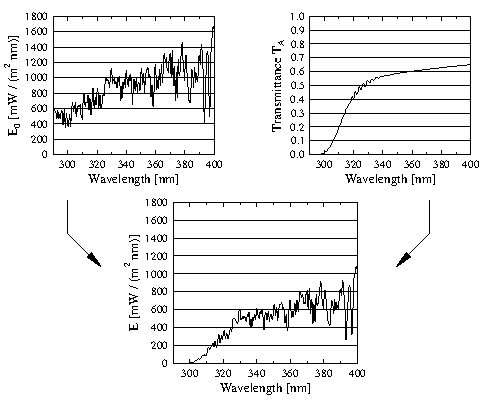
\includegraphics[width=1.\hsize]{figs/transpz.pdf}
  \caption{{\sl uvspec} calculation of spectral irradiance in the
    ultraviolet range. (Top left) High-resolution extraterrestrial irradiance
    \citet{kurucz92}, averaged over 0.1 nm intervals. 
    (Top right) Low-resolution atmospheric
    transmittance for US standard 
    atmosphere, solar zenith angle 0$^\circ$. 
    (Bottom) Product of both: spectral irradiance.}
  \label{fig:transpz}
\end{figure}

The transmittance (or reflectance) is calculated on a moderate
resolution grid which reduces the number of calls to the
\code{rte\_solver} and hence the computational time. Then, the
transmittance is interpolated to the wavelengths in the
\code{source solar file} (which is usually defined with higher spectral
resolution), multiplied with the extraterrestrial irradiance, and
possibly post-processed.  Hence, the wavelength in the output spectrum
are those contained in the \code{source solar file} which has two important
implications: (1) Only those wavelengths are output that are contained
in the \code{source solar file}. If e.g. a monochromatic calculation is
defined by setting '\code{wavelength 327.14}', there will only be
output if the wavelength 327.14 is explicitely listed in
\code{source solar file}; (2) this is also true at thermal wavelengths where
the extraterrestrial irradiance is zero; hence, even for a calculation
in the thermal range a \code{source thermal file} can be specified which
defines the output grid in the first column and arbitrary values in
the second column. Keeping these points in mind, \code{source solar/thermal file} is
a convenient way to define an arbitrary output
grid. \code{file} may be omitted for thermal radiation
calculations (\code{source thermal}), representative wavelength 
calculations (\code{mol\_abs\_param reptran}), as well as for
\code{output\_quantity transmittance} and \code{output\_quantity reflectivity} calculations. 
If omitted, the output grid equals the internal wavelength grid.

If required, a {\bf user-defined internal grid} can be specified with
\code{wavelength\_grid\_file} or \code{mol\_tau\_file abs}. Note
that this is a way to speed up the calculation considerably. E.g., for
some applications the internal grid in the UV-A and visible can be set
to 10nm which would reduce computational times by up to a factor of
10.

Things are completely different if a k distribution method is selected 
(see below). In this case 
all flexibility is taken away from the user which is an inherent feature
of the k distribution method. Internal grid as well as the
extraterrestrial file are in this case defined by the choice of the
parameterization itself.

\begin{figure}[t]
  \centering
  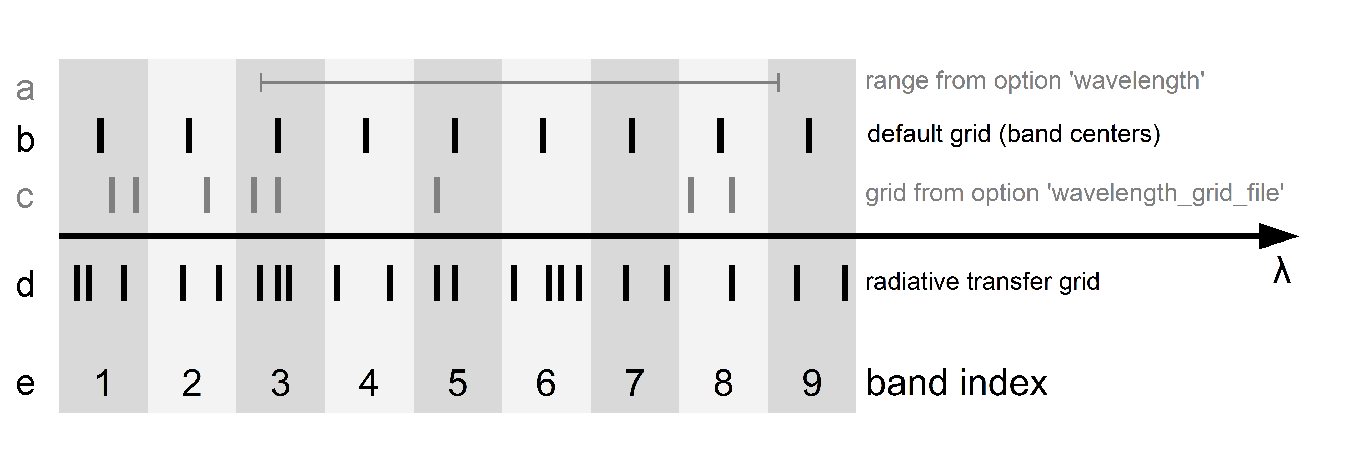
\includegraphics[width=1.\hsize]{figs/reptran_lambda_grids.pdf}
  \caption{Example for internal wavelength grids when using \codeidx{mol\_abs\_param reptran} (see text for details); 
     the shaded areas illustrate the spectral ranges of the different parameterized adjacent non-overlapping bands.}
  \label{fig:reptran_grid}
\end{figure}

If the band parameterization REPTRAN is used, two internal grids exist, 
as illustrated in Fig.~\ref{fig:reptran_grid}:
The first internal grid (above arrow) by default is defined by the wavelengths at the centers of the bands (line b of Fig.~\ref{fig:reptran_grid}).
The wavelength range is selected using the \codeidx{wavelength} option (line a of Fig.~\ref{fig:reptran_grid}); 
all bands overlapping with the specified wavelength range are modeled, for example bands 3 to 9 in Fig.~\ref{fig:reptran_grid}.
The first internal grid can be specified directly by the user with \codeidx{wavelength\_grid\_file} option (line c of Fig.~\ref{fig:reptran_grid}). 
The second internal grid consists of the representative wavelengths where the radiative transfer calculations are performed (line d of Fig.~\ref{fig:reptran_grid}).
The representative wavelengths grid is created automatically for all bands required for the first internal grid; 
for example, the second internal grid contains only the representative wavelengths required for bands 1, 2, 3, 5, and 8 for the \codeidx{wavelength\_grid\_file} illustrated in line c of Fig.~\ref{fig:reptran_grid}.
After the radiative transfer calculations are finished, transmittances calculated 
at the second internal grid are converted to transmittances at the first internal grid according to
the weighting given by the parameterization. The transmittances at the first internal grid
are used for further processing, i.e. to calculate the results on the output grid.

\subsection{Spectral resolution}

{\sl uvspec} offers five different ways of spectral calculations:
\begin{enumerate}
\item \strong{Spectrally resolved calculation} in the UV and visible
spectral ranges;
\item \strong{Line-by-line calculation} with user-defined molecular
absorption data;
\item \strong{The correlated-k method};
\item \strong{Representative wavelengths} parameterization for spectral 
  calculations and satellite channels as described by \citet{gasteiger2014};
  {\sl uvspec} uses this approach by default;
\item \strong{Pseudo-spectral calculation} with exponential-sum-fit,
from LOWTRAN; code adopted from SBDART \citep{Ricchiazzi1998b}.
\end{enumerate}

The choice of the method is determined by the problem and the decision
is therefore entirely up to the user. The spectrally resolved
calculation and the line-by-line calculation are more or less exact
methods while the correlated-k distribution, the pseudo-spectral
calculation, and representative wavelength method are 
approximations that provide a compromise between speed
and accuracy. In the following it is briefly described which method
fits which purpose:

A \strong{spectrally resolved calculation} is the most straightforward
way, and is a good choice for all users interested in the
ultraviolet and visible spectral ranges. This method is activated by the 
input option \code{mol\_abs\_param crs}. In the UV/VIS gas absorption
generally occurs in broad bands with only slow spectral variation, the
most important of these being the Hartley, Huggins, and Chappuis bands
of ozone. Hence, a radiative transfer calculation every 1nm usually is
sufficient to fully resolve any spectral variation using the method
described in the last section. Absorption cross sections for various
species are included, among them the most important O3 and NO2.

In the infrared, however, molecular absorption spectra are
characterized by thousands of narrow absorption lines. There are two
ways to treat these, either by highly resolved spectral calculations,
so-called \strong{line-by-line} calculations, or by a band
parameterization. Concerning line-by-line, {\sl uvspec} offers the
possibility to define a spectrally resolved absorption cross section
profile using \code{mol\_tau\_file abs}. There is no option in
libRadtran to generate such a \code{mol\_tau\_file abs}, because (1)
the HITRAN database which forms the basis for such calculations
amounts to about 100 MByte which are updated continuously; and (2),
there are sophisticated line-by-line programs available, like
e.g. ARTS \citep{eriksson2011}. Using ARTS it is
straightforward to create the input for {\sl uvspec} line-by-line
calculations since it provides an option to write the absorption optical
thicknesses in the required format. Line-by-line cross sections
available for the six standard profiles that come with libRadtran are
also available on request. Figure~\ref{fig:lblo2a}
shows an example of a line-by-line calculation of the
atmospheric transmittance in two selected solar and thermal spectral
ranges, the O2A-absorption band around 760~nm and a region within the
infrared window around 10~$\mu$m.

\begin{figure}
  \centering
  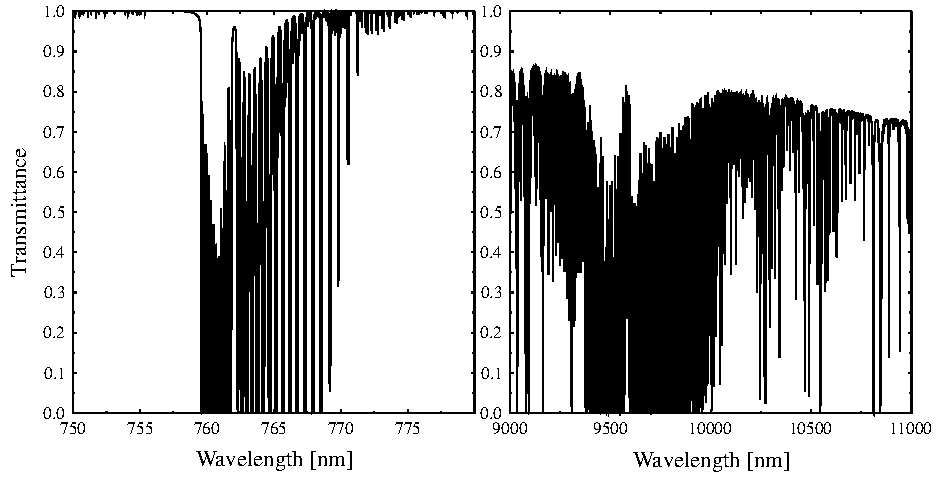
\includegraphics[width=1.0\hsize]{./figs/lblo2a.pdf}
  \caption{Line-by-line calculation of the
    atmospheric transmittance in two selected solar and thermal spectral
    ranges, the O2A-absorption band around 760~nm and a region within the
    infrared window around 10~$\mu$m.}
  \label{fig:lblo2a}
\end{figure}

All spectral lines in the left figure are due to absorption by oxygen,
while the ones in the right figure are due to ozone, water vapour, and
CO2. Line-by-line is obviously the exact way for radiation
calculations. For most applications, however, line-by-line is far too
slow. Here one needs a band parameterization.
{\sl uvspec} contains several {\bf correlated-k
parameterizations} which are invoked with \code{mol\_abs\_param}, in
particular \citet{Kato1999b, fu92, Kratz1995}, as
well as the possibility to specify a user-defined
one. \citet{Kato1999b}
is a accurate parameterization for the solar spectral
range. {\sl uvspec} contains three different versions:
\begin{description}
\parameter{Kato}
The original tables provide by Seiji
Kato which should correspond to the full version described in Kato et
al. (1999); 575 subbands total, that is, 575 calls to the
\code{rte\_solver}
\parameter{Kato2}
A new, optimized version of the
tables, provided by Seiji Kato, 2003, with only 148 subbands (that is,
calls to the \code{rte\_solver}); the uncertainty is only slightly
higher than \code{Kato}; the absorption coefficients are based on
HITRAN 2000.
\parameter{Kato2.96}
Similar to \code{Kato2} but based on HITRAN96.
\end{description}

Figure~\ref{fig:figure3} shows a comparison between the
three parameterization which are part of libRadtran and the data from
Figure 3 by \citet{Kato1999b}. It is immediately obvious that the
uncertainty is high for all bands above 2.5 micrometer which is
probably due to the treatment of band overlap. For this reasons, the
results for the indiviudal bands should not be trusted while the
integrated shortwave radiation (the sum of all 32 bands) is calculated
with high accuracy because (1) the bands above 2.5 micrometer
contribute only little to the integrated irradiance; and (2) errors
are random and cancel each other to some degree.

\begin{figure}[t]
  \centering
  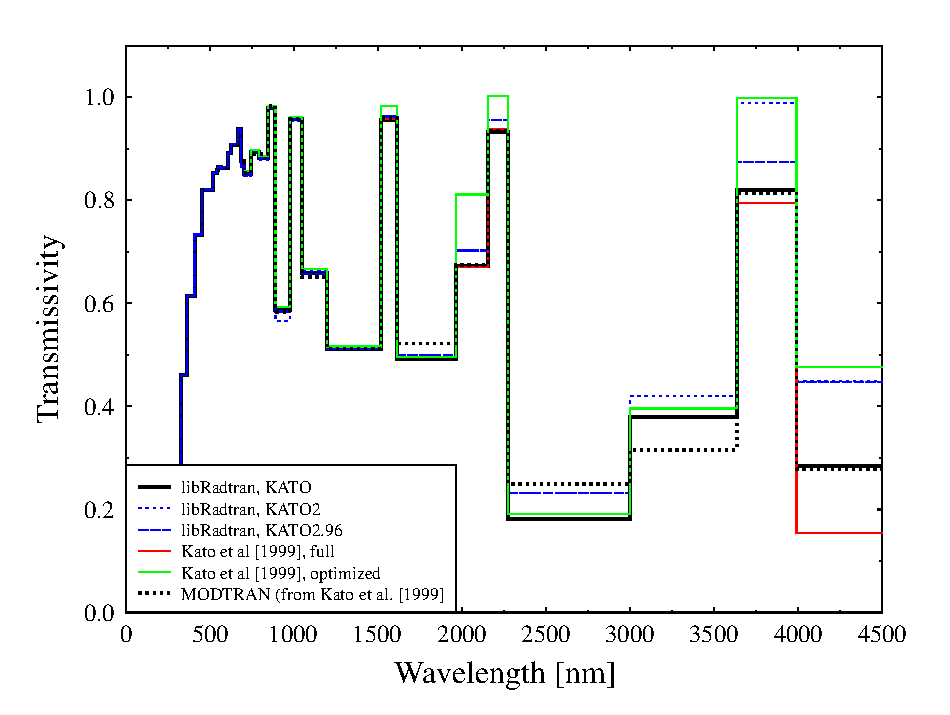
\includegraphics[width=1.0\hsize]{./figs/figure3.pdf}
  \caption{Comparison between the three parameterization which are
    part of {\sl uvspec} and the data from Figure 3 by \citet{Kato1999b}.}
  \label{fig:figure3}
\end{figure}

For more information on these parameterizations please refer to the
mentioned publications. Correlated-k is a powerful way to calculate
spectrally integrated quantities, however, it takes away some
flexibility. In particular, this means that the wavelength grid is no
longer chosen by the user but by the parameterization, that is, by
{\sl uvspec}. The {\sl uvspec} output is then no longer spectral
quantities, e.g. W/(m$^2$nm), but integrated over the spectral bands,
e.g. W/m$^2$.

A simple but complete example for a correlated-k approximation of the
solar spectrum:

\efile{../examples/UVSPEC_KATO.INP}

Here, the solar spectrum is split up into 32 bands according to
\citet{Kato1999b}.
In order to calculate integrated shortwave irradiance,
simply sum the outputs, or even simpler, add \codeidx{output\_process sum} to the
input file.

As an molecular absorption parameterization, we have implemented the 
\strong{representative wavelength approach} (REPTRAN) in the solar and thermal spectral range.
REPTRAN is used as the default spectral approach in {\sl uvspec}.
Parameterized bands are available for spectral calculations.
Furthermore a number of satellite channels have been parameterized in addition 
(available with \code{mol\_abs\_param reptran\_channel}).
The approach is described by \citet{buehler2010} and \citet{gasteiger2014}.
The required data files are available at the libRadtran homepage.
Band- and channel-integrated quantities are parameterized by weighted sums of these quantities 
calculated at a few representative wavelengths.
Solar bands are parameterized in the spectral range from 395~nm to 5000~nm, thermal bands from 2.5~$\mu$m to 100~$\mu$m.
For both solar and thermal bands different spectral resolutions are available and can be selected using 
\code{mol\_abs\_param reptran coarse|medium|fine} (default: \code{coarse}). \code{fine} corresponds to a band width of 1~cm$^{-1}$, 
whereas widths of 5~cm$^{-1}$ and 15~cm$^{-1}$ are used by \code{medium} and \code{coarse}, respectively.
The solar band parameterizations are extended by 15~cm$^{-1}$ wide bands from 240~nm to 395~nm, where only a single representative 
wavelength (band center) is used for each band.

\begin{figure}
  \centering
  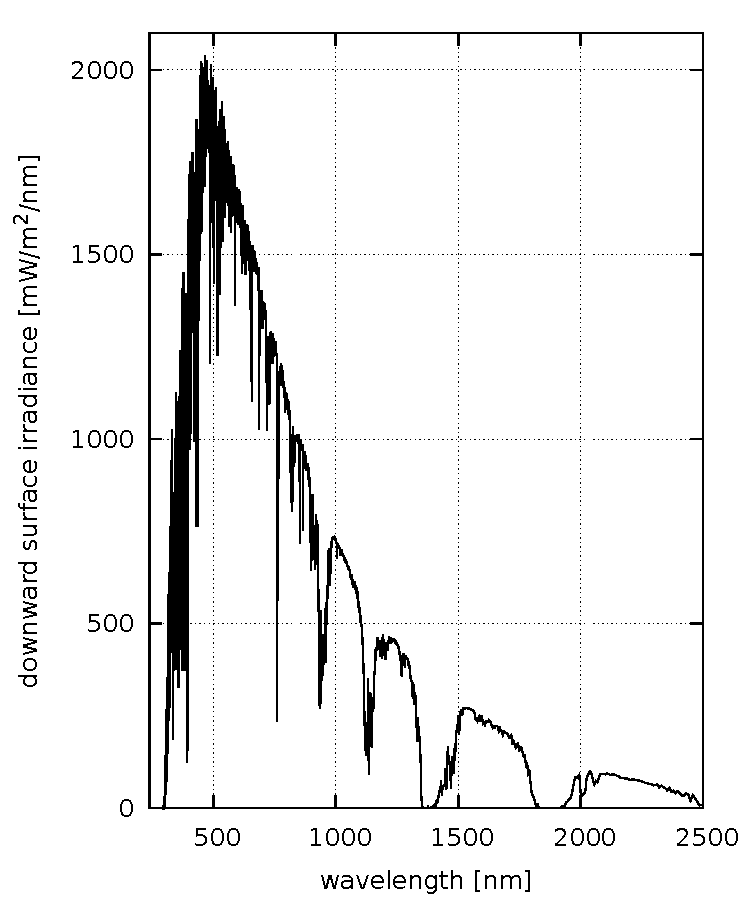
\includegraphics[width=0.49\hsize]{./figs/reptran_solar.pdf}
  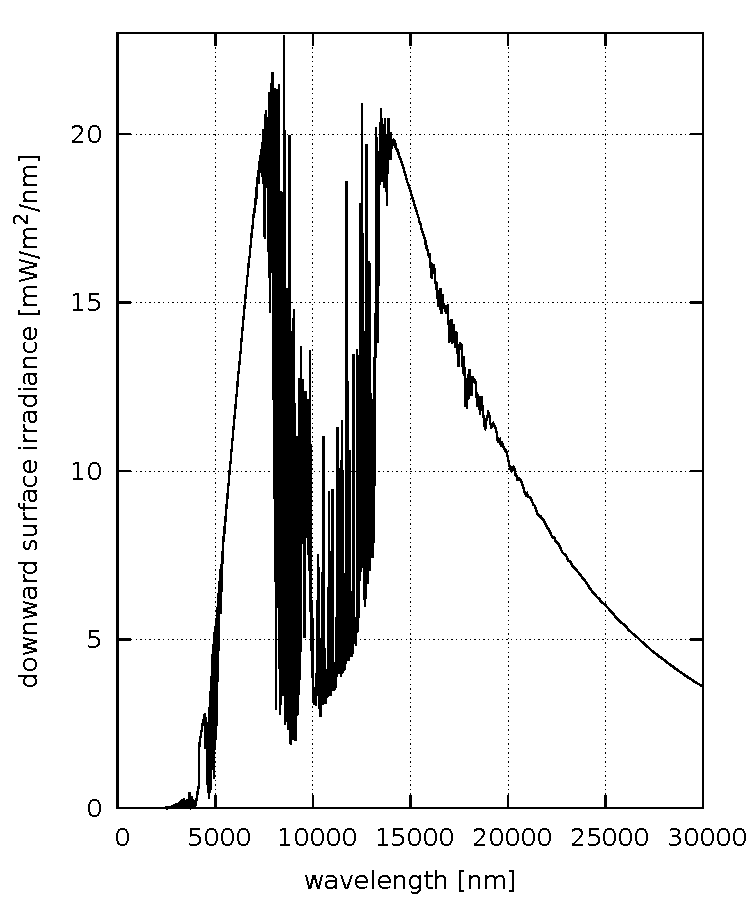
\includegraphics[width=0.49\hsize]{./figs/reptran_thermal.pdf}
  \caption{Results of solar and thermal calculations using \code{mol\_abs\_param reptran} for US standard atmosphere.} 
  \label{fig:reptran}
\end{figure}

Figure~\ref{fig:reptran} shows the results of solar and thermal
calculations from 395~nm to 100~$\mu$m. The water vapour absorption bands in the solar range are
clearly visible, as is the absorption window around 10~$\mu$m in
the thermal. 

An example which calculates fluxes at the ground in the solar range is available in \code{examples/UVSPEC\_REPTRAN\_SOLAR.INP}:

\efile{../examples/UVSPEC_REPTRAN_SOLAR.INP}

Internally, the extraterrestrial flux from \citet{kurucz92} is applied, thus no \code{source solar file} is required.

The default unit for solar fluxes is mW/(m$^2$nm), and for thermal fluxes is W/(m$^2$cm$^{-1}$).
Band-integrated quantities are obtained using the option \code{output\_process per\_band}.
The sum over all bands can be calculated using the option \code{output\_process sum}.

The example \code{examples/UVSPEC\_REPTRAN\_THERMAL.INP} calculates brightness temperatures of band-integrated radiances in the thermal range
from different viewing zenith angles at top of atmosphere:

\efile{../examples/UVSPEC_REPTRAN_THERMAL.INP}

Fig.~\ref{fig:o2a} compares the spectral resolutions of REPTRAN and LOWTRAN.
The spectral resolutions are equal for LOWTRAN and REPTRAN medium (5~cm$^{-1}$). 
However spectral information was 
``degraded to 20~cm$^{-1}$ resolution for use in LOWTRAN'' \citep{Ricchiazzi1998b} with the effect that LOWTRAN spectra
are significantly smoother than REPTRAN medium spectra.

Finally, the example \code{examples/UVSPEC\_REPTRAN\_CHANNEL\_THERMAL.INP} calculates the thermal brightness temperatures of a channel of a MSG satellite centered at $\lambda$=3.9$\mu$m looking at different viewing zenith angles:

\efile{../examples/UVSPEC_REPTRAN_CHANNEL_THERMAL.INP}

This setup is the same as in the previous input file whereby channel integrals are calculated instead of band integrals (\code{mol\_abs\_param reptran} of the included file is overwritten by \code{mol\_abs\_param reptran\_channel} here).
The available channels are listed in \code{data/correlated\_k/reptran/channel\_list.txt}.

Though we recommend REPTRAN for spectral calculations, the molecular absorption parameterization from
LOWTRAN/SBDART by \citet{Ricchiazzi1998b} is available mainly for compatibility reasons.
LOWTRAN allows for \strong{pseudo-spectral calculations} in the whole spectral range, the respective 
section of this paper says:

\begin{quotation} 
  SBDART relies on low-resolution band models
  developed for the LOWTRAN 7 atmospheric trans-mission code (Pierluissi
  and Peng, 1985).
  These models provide clear-sky atmospheric
  transmission from 0 to 50000 cm-1 and include the effects of all
  radiatively active molecular species found in the earth s
  atmosphere. The models are derived from detailed line-by-line
  calculations that are degraded to 20 cm-1 resolution for use in
  LOWTRAN. This translates to a wavelength resolution of about 5 nm in
  the visible and about 200 nm in the thermal infrared. These band
  models represent rather large wavelength bands, and the transmission
  functions do not necessarily follow Beers Law. This means that the
  fractional transmission through a slab of material depends not only on
  the slab thickness, but also on the amount of material penetrated
  before entering the slab. Since the radiative transfer equation solved
  by SBDART assumes Beers Law behavior, it is necessary to express the
  transmission as the sum of several exponential functions (Wiscombe and
  Evans, 1977). SBDART uses a three-term exponential fit, which was also
  obtained from LOWTRAN 7. Each term in the exponential fit implies a
  separate solution of the radiation transfer equation. Hence, the RT
  equation solver only needs to be invoked three times for each spectral
  increment. This is a great computational economy compared to a higher
  order fitting polynomial, but it may also be a source of significant
  error.
\end{quotation}

The LOWTRAN/SBDART gas parameterization is invoked with
\code{mol\_abs\_param LOWTRAN}. The spectral resolution may be
arbitrarily chosen by the user. If not explicitely defined with
\code{wavelength\_grid\_file}, an internal grid with a step width of
0.5nm below 350nm and 1nm above 350nm is chosen which is practically
overkill for most applications in the infrared. An extraterrestrial
spectrum covering the complete solar range is provided at two
different resolutions, \code{data/solar\_flux/kurudz\_1.0nm.dat} and
\code{data/solar\_flux/kurudz\_0.1nm.dat}. An example for the solar
range is shown in \code{examples/UVSPEC\_LOWTRAN\_SOLAR.INP}:

\efile{../examples/UVSPEC_LOWTRAN_SOLAR.INP}

while \code{examples/UVSPEC\_LOWTRAN\_THERMAL.INP} shows how to do a
thermal calculation:

\efile{../examples/UVSPEC_LOWTRAN_THERMAL.INP}

Please note the following points:
\begin{itemize}
\item Thermal radiation is per default output in W/(m$^2$cm$^{-1}$), if the
  bandwidth is equal to 1~cm$^{-1}$ (default for \code{mol\_abs\_param LOWTRAN}
  calculations). Otherwise the output is the integrated flux over the
  wavenumber interval specified by \code{thermal\_bandwidth},
  \code{thermal\_bands\_file}, or by the \code{mol\_abs\_param} option
  (Kato, Kato2, Kato2.96, Fu, AVHRR\_KRATZ, or Generic). To convert
  e.g. to W/(m2 nm) use \code{output\_process per\_nm} or multiply with k/lambda
  where k is the wavenumber [cm$^{-1}$] and lambda is the wavelength [nm]. To
  calculate band-integrated thermal quantities please consider
  \codeidx{thermal\_bands\_file}.
\item Even though no extraterrestrial irradiance is required, a
  \code{source thermal file} may be specified for the thermal case. The reason
  is that, as explained initially, the \code{source thermal file} defines the
  output grid. The second column in \code{source thermal file} can be chosen
  arbitrarily in this case because it is ignored.
\item For the choice of the wavelength grid for the calculation
  (\code{wavelength\_grid\_file}) please consider that the resolution
  of the absorption parameterization is 5~cm$^{-1}$ which translates to 0.3nm
  at 750~nm and to 50~nm at 10~$\mu$m. Choosing higher resolutions for
  the internal wavelength grid (\code{wavelength\_grid\_file}) is
  usually a waste of computational time.
\item Please also make sure to choose a fine enough spectral
  resolution in order to capture all absorption features.
\end{itemize}

\begin{figure}
  \centering
  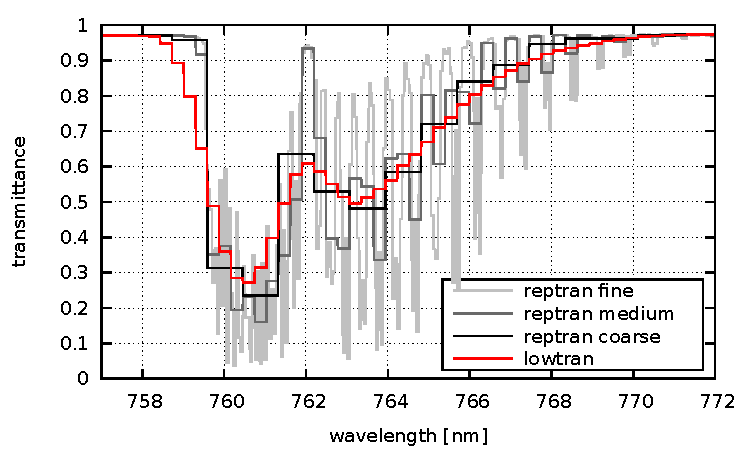
\includegraphics[width=1.0\hsize]{figs/resolution_o2a.pdf}
  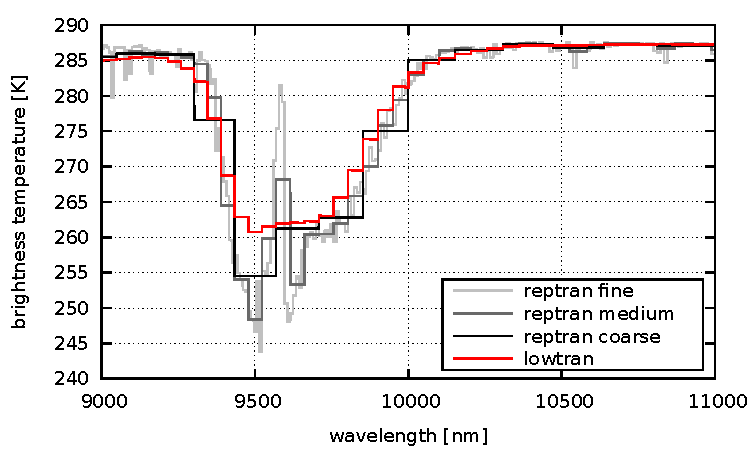
\includegraphics[width=1.0\hsize]{figs/resolution_o3.pdf}
  \caption{Two selected wavelength intervals in the
    solar range (upper panel, O2A band) and the thermal range 
    (lower panel, O3 band at $\lambda\approx9.6\mu$m), to demonstrate the spectral resolution of the
    LOWTRAN and REPTRAN absorption parameterizations.}
  \label{fig:o2a}
\end{figure}

The red curve in Fig.~\ref{fig:o2a} demonstrates the spectral resolution of the LOWTRAN/SBDART 
absorption parameterization (and REPTRAN, see above)
for two selected wavelength intervals of the solar and thermal range.
The resolution of LOWTRAN is about 5~cm$^{-1}$ which translates to about 0.3~nm in the
left figure (oxygen A-band) and 50nm in the right figure (ozone
absorption band in the atmospheric window). Compare this figure to the
above line-by-line example to get an impression about the differences
between the methods.


\subsection{Aerosol}
\index{Aerosol}
All options to set up and modify aerosol properties start with
\code{aerosol\_}.  Aerosols may be specified in a hierarchical
way. The most simple way to define an aerosol is by the command
\codeidx{aerosol\_default} which will set up the aerosol model by
\citet{shettle89}. The default properties are a rural
type aerosol in the boundary layer, background aerosol above 2km,
spring-summer conditions and a visibility of 50km. These settings may
be modified with \codeidx{aerosol\_haze}, \codeidx{aerosol\_vulcan},
\code{aerosol\_season}, and \codeidx{aerosol\_visibility}. More
information can be introduced step by step, overwriting the default
parameters. \codeidx{aerosol\_file tau}, \codeidx{aerosol\_file ssa}, and
\codeidx{aerosol\_file gg}, can be used to define the profiles of
optical thickness, single scattering albedo, and asymmetry
parameter. The integrated optical thickness can be set to a constant
value using \codeidx{aerosol\_modify tau set} or scaled with
\codeidx{aerosol\_modify tau scale}. The single scattering albedo may be scaled
by \codeidx{aerosol\_modify ssa scale} or set to a constant value by
\codeidx{aerosol\_modify ssa set}.  The aerosol asymmetry factor may be set by
\codeidx{aerosol\_modify gg set}. The wavelength dependence of the aerosol
optical depth is specified using the \codeidx{aerosol\_angstrom}
parameter. \codeidx{aerosol\_file moments} allows specification of the
scattering phase function. If microphysical properties are available
these may be introduced by defining the complex index of refraction
\codeidx{aerosol\_refrac\_index} and the
size distribution \codeidx{aerosol\_sizedist\_file}. Finally, one may
define the aerosol optical properties of each layer explicitely using
\codeidx{aerosol\_file explicit}.

The following list is an overview of some aerosol description
parameters. The entries are arranged in a way that a parameter
'overwrites' all values higher up in the list.

\begin{description}
  \parameter{aerosol\_default} 
  Generate default aerosol according to \citet{shettle89}.
  \parameter{aerosol\_vulcan, aerosol\_haze, aerosol\_season,
    aerosol\_visibility}
  Set \cite{shettle89} aerosol properties (aerosol
  type, visibility)
  \parameter{aerosol\_file explicit}
  Specify optical properties of each
  layer explicitly, that is, extinction coefficient, single scattering
  albedo, and the moments of the phase function (everything as a
  function of wavelength).
  \parameter{aerosol\_file tau , aerosol\_file ssa,
    aerosol\_file gg}
  Overwrite profiles of optical thickness, single
  scattering albedo, and asymmetry parameter
  \parameter{aerosol\_file moments}
  Specify a phase function to be
  used instead of the Henyey-Greenstein phase function
  \parameter{aerosol\_refrac\_index, aerosol\_sizedist\_file}
  Calculate optical properties from size
  distribution and index of refraction using Mie theory. Here is an
  exception from the rule that ALL values defined above are overwritten
  because the optical thickness profile is re-scaled so that the optical
  thickness at the first internal wavelength is unchanged. It is done
  that way to give the user an easy means of specifying the optical
  thickness at a given wavelength.
  \parameter{aerosol\_species\_file} Define profiles of arbitrary aerosol
  types. The profiles will be mixed within {\sl uvspec}. Optical properties
  of the aerosol types can be provided using the option
  \code{aerosol\_species\_library}. One library may be downloaded from
  \url{www.libradtran.org}, it inlcudes aerosol optical properties
  based on size distribution parameters and refractive indices from
  the OPAC database \citep{hess98:_optic_proper_aeros_cloud}. The optical properties
  have been generated using the \code{mie} tool and they include full
  phase matrices, e.g. they are suitable for calculations with
  polarization.  
  \parameter{aerosol\_modify gg/ssa/tau scale/set}
  Overwrite
  profiles of asymmetry parameter and single scattering albedo
  \parameter{aerosol\_angstrom}
  Overwrite the integrated optical
  thickness (profiles are not changed).
\end{description}

An example for a {\sl uvspec} aerosol description is

\efile{../examples/UVSPEC_AEROSOL.INP}

\noindent By combining this with the clear sky example given above a
complete {\sl uvspec} input file including aerosol is constructed.


\subsection{Water clouds \label{seq:wc}}
\index{Water clouds}

All options to set up and modify water cloud properties start with
\code{wc\_}.

The easiest way to define a water cloud is to specify a
\code{wc\_file} which defines the liquid water content and effective
droplet radius at each model layer or level. By combining the
following lines with the clear sky example given above a complete
{\sl uvspec} input file including water clouds is constructed.

\efile{../examples/UVSPEC_WC.INP}

A typical example for a wc\_file looks like:

\begin{Verbatim}[fontsize=\footnotesize, frame=single] 
# z LWC R_eff 
# (km) (g/m3) (um) 
5.000 0 0 
4.000 0.2 12.0 
3.000 0.1 10.0 
2.000 0.1 8.0
\end{Verbatim}

The three columns are the level altitude [km], the liquid water
content [g/m$^3$], and the effective droplet radius [micrometer]. Per
default (since version 1.4), these quantities are interpreted as layer
quantities, and in the above example, the cloud would extend from 2 to
5~km, with e.g. a LWC of 0.2~g/m$^3$ for the layer between 4 and
5~km. Before version 1.4 the \codeidx{wc\_file} was interpreted as level
quantities (unless \codeidx{wc\_layer} was specified). That is, the value
0.2~g/m$^3$ referred to altitude 4.0~km, as e.g. in a radiosonde
profile. The properties of each layer were calculated as average over
the adjacent levels. E.g. the single scattering properties for the
model layer between 3 and 4~km were obtained by averaging over the two
levels 3~km and 4~km. To allow definition of sharp cloud boundaries,
clouds were only formed if both liquid water contents above and below
the respective layer were larger than 0. Hence, in the above example,
the layers between 2 and 3 as well as between 3 and 4~km were cloudy
while those between 1 and 2km and between 4 and 5~km were not. To
switch to the old behaviour, use \codeidx{interpret\_as\_level wc}.

To make sure that the clouds really look as you want them to look, it
is recommended to use the \codeidx{verbose} option. This option shows not
only where the cloud is actually placed, it rather tells the user
exactly how LWC and effective radius are translated into optical
properties, depending on the choice of parameterisation. Please also
note that the definition of the empty top level at 5km is important to
tell {\sl uvspec} where the cloud ends. If omitted, the cloud would
extend all the way to the top of the atmosphere.

There are different ways to convert the microphysical properties to
optical properties. Either a parameterization is used, like the one by
\citet{Hu1993} (which is the default), or by Mie
calculations. The latter are very time-consuming, hence we decided not
to include these online into {\sl uvspec} but rather have an option
to read in pre-calculated Mie tables. The option \codeidx{wc\_properties}
controls the method: \code{hu} selects the \citet{Hu1993}
parameterization, \code{mie} selects pre-calculated Mie tables which
are available at \url{http://www.libradtran.org}. The tables include
the full scattering phase matrices and can therefore be used for
polarization dependent calculations. If \code{wc\_properties
mie} is selected, the model expects one or more Mie cloud property
files including each internal wavelength which is useful for the fixed wavelength
grids used by the correlated-k parameterisations \code{mol\_abs\_param
kato}, \code{mol\_abs\_param fu}, etc. For a spectral calculation with
free wavelength grid, there is also the possibility to use a
pre-defined set of Mie tables (available at the web site) and to
define \code{wc\_properties mie interpolate} to automatically
interpolate the Mie properties to the internal wavelength
grid. Although this is an extremely useful option, please use it
careful because it might consume enourmous amounts of memory. Finally,
there is the option to define an arbitrary file which can be generated
using the \codeidx{mie} tool (see section~\ref{sec:optprop}).

As for the aerosol, there are several options to modify the optical
properties of the clouds. And of course there is also the option of
defining all cloud properties explicitely using \code{wc\_file moments}.

\subsection{Ice clouds \label{seq:ice_clouds}}
\index{Ice clouds}

Ice clouds are generated in a similar way to water clouds.  All
options to set up and modify ice cloud properties start with
\code{ic\_}. The main difference between water and ice clouds is that
the latter usually consist of non-spherical particles. Hence, the
conversion from microphysical to optical properties is much less
defined, and several parameterizations are available. Please note in
addition that there are different definitions of the effective radius.
E.g. the parameterizations by \citet{Key2002} and
\citet{baum05b:_bulk, baum07:_bulk} use the same definition whereas 
\citet{Fu1996} actually
uses another definition (see explanation of
\codeidx{ic\_properties}). Finally, the sharp forward peak which is
typical for ice particles can also be treated differently: E.g.,
\citet{Fu1996} provides delta-scaled optical properties while
\citet{Key2002} uses unscaled parameters (see explanation of
\codeidx{ic\_fu deltascaling}). Figure~\ref{fig:fuyang} illustrates the
implications.  Plotted are extinction coefficient, asymmetry
parameter, and single scattering albedo for ice clouds with an
effective radius of 25 micrometers as a function of wavelength. If
treated consistently, all parameterizations \citet{Key2002},
\citet{Fu1996}, and \citet{baum05b:_bulk, baum07:_bulk} provide nearly
identical results (solid 
lines, default settings in {\sl uvspec}).  If the definition of
effective radius by \citet{Fu1996} and delta-scaling is applied the optical
properties look different. The effect of delta scaling on a radiative
transfer calculation is that the direct irradiance in increased and
the diffuse irradiance is decreased, whereas the global irradiance
remains unchanged.  The definition of the effective radius has a
smaller effect but it modifies also the global irradiance.  Note that
the parameterization by \citet{baum05b:_bulk, baum07:_bulk} is plotted only up
to 2200~nm. The reason is that it does not cover the full spectral
region, it is available for two spectral regions (from 0.4--2.2~$\mu$m
and from about 3--100~$\mu$m).
For the calculation of radiances one should use either
\code{ic\_properties baum}, \code{hey}, \code{baum\_v36} or
\code{yang2013} because these parameterizations include complete
scattering phase functions and do not use approximations like the
Heney-Greenstein phase function.  \code{hey}, \code{baum\_v36} and
\code{yang2013} can also be used for polarized radiative transfer. The
data needed for \code{baum}, \code{hey}, \code{baum\_v36}, and
\code{yang2013} is available at \url{www.libradtran.org}.

\begin{figure}
  \centering
  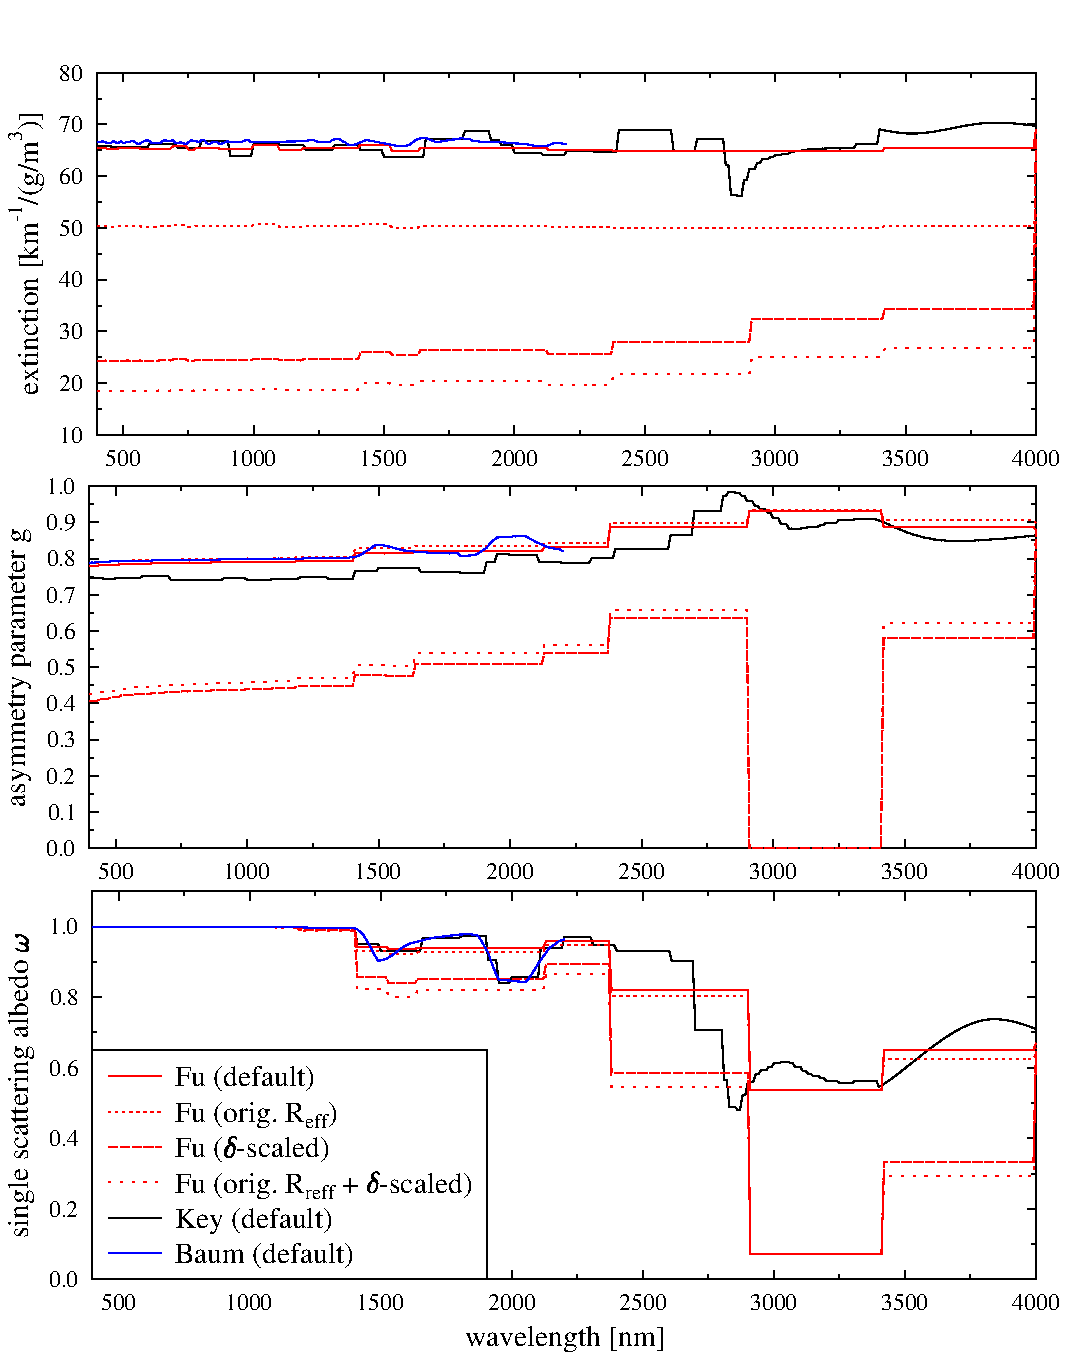
\includegraphics[width=1.0\hsize]{./figs/fuyang.pdf}
  \caption{Extinction coefficient, asymmetry
    parameter, and single scattering albedo for ice clouds with an
    effective radius of 25~$\mu$m as a function of wavelength for
    various parameterizations.}
  \label{fig:fuyang}
\end{figure}

\subsection{Calculation of radiances}
\index{radiances}

To calculate radiances the following lines will do the job when
combined with the clear sky example above

\efile{../examples/UVSPEC_RADIANCES.INP}

In this example radiances are calculated for the specified directions,
where \code{umu} are the cosines of the viewing zenith directions and
\code{phi} are the viewing azimuth angles.

\ifmystic{
  The following examples shows a complete input file for the calculation
  of polarized radiances using MYSTIC:
  \efile{../examples/UVSPEC_MC_POL.INP}
  This example is only for a 1D clear sky atmosphere. For radiance
  calculations it is strongly recommended to use the local estimate
  method (\codeidx{mc\_escape}, e.g. \citet{marshak2005}) which
  significantly reduces the noise in the results. Further, for
  radiance calculations in the presence of clouds or any other
  particle type with strong forward scattering peak, we strongly
  recommend to use the variance reduction technique VROOM
  (\codeidx{mc\_vroom}, \citet{buras2011a}).} \ifthreedmystic{In order to
  include 3D clouds, a 2D surface albedo, a 2D BRDF, or topography please
  refer to the MYSTIC documentation in section~\ref{sec:mystic}. 
  }

%\subsection{More examples}

%More examples with output are found in the \file{examples} directory.
%Several examples are also availabe through the
%{\sl uvspec} Graphical User Interface (see \file{GUI} directory).       



%--- Calculation of optical properties
\chapter{Calculation of optical properties - \code{mie}}
\label{sec:optprop}

\index{Mie}

{\sl libRadtran} includes the tool \code{mie} to calculate optical
properties of spherical particles. Two different efficient and well
tested Mie codes are implemented: The
one by \citet{wiscombe80a} and the one by \citet{bohren1998}. Scattering phase matrices and
corresponding Legendre polynomials can currently only be calculated
using the code by \citet{wiscombe80a}.

\section{Basic usage}

\subsection{Running \code{mie}}

Mie scattering calculations are performed for a specified
wavelength interval. The \code{mie} program reads input from standard input, 
and outputs to standard output or to a file. If
\code{output\_user netcdf} is specified \code{mie} generates a file
that can be used for radiative transfer calculations with
\code{uvspec}.

The \code{mie} tool is normally invoked in the following
way: 

\begin{Verbatim}[fontsize=\footnotesize]   
  mie < input_file > output_file 
\end{Verbatim}

\strong{Warning:} Please note the error checking on input variables 
is very scarce at the moment. Hence, if you provide erroneous input, 
the outcome is unpredictable.

\subsection{The \code{mie} input file}

The \code{mie} input file consists of single line entries, each making
up a complete input to the mie program. First on the line comes
the parameter name, followed by one or more parameter values. The 
parameter name and the parameter values are seperated by white space.

Filenames are entered without any surrounding single or double quotes.

Comments are introduced by a \code{\#}. Blank lines are ignored.

\subsection{Model output}

The standard output (stdout) of the mie program is one line for each 
wavelength and each effective radius.
The format of the output line is
\begin{Verbatim}[fontsize=\footnotesize, frame=single, samepage=true]   
  lambda refrac_real refrac_imag qext omega gg spike pmom
\end{Verbatim}
The keywords here are the same as in input option
\code{output\_user}. The Legendre polynomials \code{pmom} are only
caclulated if the option \code{nmom} is specified.

If \code{output\_user netcdf} is specified the output is written to a
netcdf file in the format that is required by \code{uvspec}.

\section{Examples}

\subsection{Calculation for one particle}

The following example shows a Mie calculation for a single spherical
particel with a radius of 200~$\mu$m. The refractive index is
specified by the user. The calculation is performed for wavelengths
from 280 to 5000~nm in 5~nm steps.
\efile{../examples/MIE_1.INP}

\subsection{Calculation for a size distribution}

Not all cloud droplets are of one specific size. The cloud droplet
size spectrum may be represented for instance by a gamma
distribution. Gamma distributions can easily be specified using the
option \codeidx{distribution} \code{gamma} as
demonstrated in the following example:
\efile{../examples/MIE_2.INP}
The refractive index of water is taken for this calculation. In order
to generate input for \code{uvspec} Legendre polynomials and from
those the phase matrices need to be calculated. The option
\codeidx{nmom} specifies how many Legendre polynomials shall be
computed. If the selected number is too small for an accurate
representation of the phase matrix, a warning is given. If
\code{output\_user netcdf} is specified the corresponding phase
matrices are calculated from the Legendre moments. The scattering
angle grid is optimized so that the phase matrix is sampled as
accurate as possible. The option \code{nthetamax} can be used to set
an upper limit of scattering angle grid points to be used. 
This example generates a netcdf file which can directly be used in
\code{uvspec} with the options \codeidx{wc\_properties} or
\codeidx{ic\_properties}.


%%% Local Variables: 
%%% mode: latex
%%% TeX-master: t
%%% End: 


%--- Further tools
\chapter{Further tools}
\label{sec:tools}

Besides {\sl uvspec} and {\sl mie} {\sl libRadtran} provides several
small tools related to radiative transfer in the atmosphere. These
tools can be found in the \file{bin} directory. 
Some of the tools are described in this chapter.
 
Help for all tools can be obtained on the command line using the
option \code{-h}. 

\section{General tools}

\subsection{Integration - \code{integrate}}
\index{integrate}

\code{integrate} calculates the integral between limits
$x_\mathrm{min}$ and $x_\mathrm{max}$ 
by interpolating the data points (x[i], y[i]) with natural cubic
splines or linear interpolation. $x_\mathrm{min}$ and $x_\mathrm{max}$ are the minimum
and maximum values of the first column in the input file. The 
x-values in the first column must be in ascending order.

The different options to \code{integrate} are displayed when executing:

\begin{verbatim}
integrate -h
\end{verbatim}

\subsection{Interpolation - \code{spline}}
\index{spline}
\index{Interpolation}

\code{spline} interpolates discrete data points using natural cubic
splines or linear interpolation. The x-values in the first column must 
be in ascending order. 

The different options to \code{spline} are displayed when executing:

\begin{verbatim}
spline -h
\end{verbatim}

\index{conv}
\subsection{Convolution - \code{conv}}
                  
\code{conv} convolutes a spectrum with a given filter function.

The different options to \code{conv} are displayed when executing:

\begin{verbatim}
conv -h
\end{verbatim}


\index{addlevel}
\subsection{Add level to profile - \code{addlevel}}

\code{addlevel} is a simple shell script to add a level to 
an atmosphere\_file or mol\_file. It is located in the \code{src} directory.

The different options to \code{addlevel} are displayed 
when executing:

\begin{verbatim}
addlevel -h
\end{verbatim}

\subsection{Numerical difference between two files -\codeidx{ndiff}}
The Perl script \code{ndiff} calculates the relative difference between two files
containing columns of numbers (file1/file0). The first column is
not included. The calculated differences are output to stdout.
If limit is different from 0.0, the number of differences greater
than abs(maxdiff) are printed to stdout. The \code{ndiff} script is
extensively used by the \file{test/test.pl} script invoked by \code{make check}.

The \code{ndiff} script is invoked by
  \begin{Verbatim}[fontsize=\footnotesize]
      ndiff [options] file0 file1
  \end{Verbatim}
The script understands the following options
\begin{description}
   \item[--limit $<$value$>$]     The minimum value in file0 considered when
                                  counting the number of differences between file0
                                  and file1. Default is 0.0.
   \item[--maxdiff $<$value$>$]   The maximum relative difference allowed between
                                  file0 and file1. Defaut is 0.0.
   \item[--sub]                   Subtract file1 - file0 instead of division
   \item[--nox]                   First column is included
   \item[--quiet]                 The differences are not output, but the number of
                                  differences are still printed.
   \item[--help]                  Print help message.
\end{description}


\section{Tools to generate input data to and analyse output data from \code{uvspec}}

% The snowalbedo tool
\input{snowalbedo}


\index{cldprp}
\subsection{Calculate cloud properties - \code{cldprp}}

\code{cldprp} calculates wavelength-dependent cloud properties 
using one of several parameterizations.

The different options to \code{cldprp} are displayed when executing:

\begin{verbatim}
cldprp -h
\end{verbatim}

% CE: Commented cldgen since it is not clear whether it is working or not !!!

% \index{cldgen}
% \subsection{Generate model clouds - \code{cldgen}}

% \code{cldgen} generates 1D, 2D, and 3D model clouds to be used as 
% input to libRadtran / MYSTIC.

% \begin{verbatim}
% cldgen < input_file > output_file
% \end{verbatim}

% format of the input and output files are described
% below. Several realistic examples of input files are subsequently 
% given.

% \strong{Warning:} Please note the error checking on input variables 
% is very scarce at the moment. Hence, if you provide erroneous input, 
% the outcome is unpredictable.
   

% \subsubsection{The \code{cldgen} input file}

% The cldgen input file consists of single line entries, each making
% up a complete input to the cldgen program. First on the line comes
% the parameter name, followed by one or more parameter values. The 
% parameter name and the parameter values are seperated by white space.

% Filenames are entered without any surrounding single or double quotes.

% Comments are introduced by a \code{\#}. Blank lines are ignored.

% The various input parameters are described in detail below.

% \FIXME{the following should be extracted from cldgen\_lex.l}


% \subsubsection{The \code{cldgen} output}

% \subsubsection{Example}

% An example of a complete input file is

% \efile{../examples/CLDGEN.INP}

% The zenith tool
\input{zenith}

% The noon tool
\input{noon}

% The angres tool
\input{angres}

% The make_angresfunc tool
\input{make_angresfunc}

% The make_slitfunction tool
\input{make_slitfunction}

% Calculate phase function
\input{phase}

% Legendre decomposition
\input{pmom}

% automated independent pixel calculation
% \input{worldloop}

\section{Other useful tools}

\subsection{SSRadar - Single Scattering Radar \index{SSRadar}}

A simple single scattering radar simulator which assumes pure Rayleigh scattering
in a 1D plan-parallel atmosphere at water or ice spheres without molecular absorption. 
It solves the equation for the radar reflectivity factor $Z$
$$
Z = \sum_i N_i D_i^6
$$

directly from the given droplet distribution defined by discrete sampling intervalls
$\left(N_i, N_i + \Delta N\right)$ containing the droplet diameters $\left(D_i, D_i 
+ \Delta D\right)$ (\citet{Rinehart2010}).

Usage (outputfile is optional, output is printed to stdout by default):
\begin{Verbatim}[fontsize=\footnotesize]
ssradar inputfile [outputfile]
\end{Verbatim}
The simulation is defined in the input file with the following structure:
\subsubsection {First line:}
\begin{description}
\item[wavelength] The wavelength in mm.
\item[Z-Position] The vertical position of the radar in m.
\item[Zenith Angle] The zenith angle in degree, $0$ means looking straight upwards, 
$180$ means looking straight downwards, must not be $90$.
\item[Ground Altitude] Vertical position of the ground in m.
\end{description}
Notes: The ground altitude can be used to add topographic data when creating two- or 
three-dimensional radar images with multiple simulations. The signal from the ground is
set to $100$ $dBZ$.
\subsubsection{Second line:}
\begin{description}
\item[Range Gates] Number of range gates.
\item[Range Gate Length] Radial Length of a range gate in m.
\item[First Range Gate] Radial Distance of the first range gate from the radar in m.
\item[Output] Ouput format. -1 is text only, 1 is mmclx only, 0 is both.
\end{description}
Notes: The simulator takes a straight radial line from the radar into the direction defined
by the zenith angle. This line is partitioned into a number of intervals (number of 
range gates) with a fixed length (range gate length) starting at a given distance 
(first range gate) from the radar. Keep in mind that the first range gate is defined by 
its distance along that line and not by its z-position, and that the length of a range
gate is the actual geometrical length. The distinction between first range gate and position
of the radar serves to be able to only focus on the parts that are needed and it will be
further important once attenuation has been implemented. MMCLX output has been added for
easy compatibility.
\subsubsection{The following lines define the reflective layers, one line per layer:}
\begin{description}
\item[Height] Z-Position of the lower border of the layer in m.
\item[Thickness] Vertical thickness of the layer in m.
\item[Effective Radius] Effective Radius of the distribution in um.
\item[Distribution] What kind of distribution (mono, gamma, log, or a filename), for
details see \code{distribution} and \code{size\_distribution\_file} in chapter \ref{sec:mie}.
\item[Distribution Parameter] Distribution Parameter for gamma and log, for
details see \code{distribution} in chapter \ref{sec:mie}.
\item[Maximum Radius Factor] Upper radius cutoff factor for gamma and log, for
details see \code{n\_r\_max} in chapter \ref{sec:mie}.
\item[Temperature] Temperature of the layer in degree Celsius.
\item[Phase] Phase of the layer, water or ice.
\item[Liquid Water Content] Liquid Water Content of the layer in $g/m^3$
\end{description}
Notes: You can simulate supercooled liquid water down to $-34^{\circ}C$.
Reflective layers must not overlap or be below ground but can otherwise be 
configured freely. 

\subsubsection{Example Input:}
\begin{Verbatim}[fontsize=\scriptsize,frame=single]
# wvl - z-pos -   zenith angle - ground altitude
# mm  - m     -   degree       - m
  8.5   500.0       45.0        0.0
# Range Gates - RG Length - First RG - Output
# (int)         m           m          (-1,0,1)
  15            500.0       0.0        -1
# height - thickness - reff - dist - distparam - max r fact - T - phase - LWC
# m        m           um     (str)  (double)    (double)  deg C  (str)   g/m^3
  1000.0   1000.0      18.0   mono       0          0        10.  water   0.30
  2000.0    500.0      15.0   log        1.1        5         0.  water   0.10
  3000.0    500.0      12.0   gamma      7          5       -10.  water   0.05
  3500.0   2000.0      10.0   dist.dat   0          0       -20.  ice     0.02
\end{Verbatim}

\subsubsection{Example Output:}
\begin{Verbatim}[fontsize=\scriptsize,frame=single]
Wavelength: 8500 um
Height of radar: 0.000000e+00 m
Zenith Angle: 0.000000e+00
Number of Range Gates: 6
Range Gate Width: 1.000000e+03 m
First Range Gate Radial Distance: 0.000000e+00 m
First Range Gate Z-Position: 0.000000e+00 m
RG No    RG Dist [m]     RG Z-Pos [m]    Z [dBZ]
1        0.000000e+00    0.000000e+00    0.000000
2        1.000000e+03    1.000000e+03    -16.016457
3        2.000000e+03    2.000000e+03    -19.641281
4        3.000000e+03    3.000000e+03    -23.466286
5        4.000000e+03    4.000000e+03    -27.732285
6        5.000000e+03    5.000000e+03    0.000000
\end{Verbatim}



\input{read_Stamnes_tab}

  


\chapter{Complete description of input options}
\label{chap:complete-description-input-options}

%---Description of uvspec options
\input{uvspec_lex}

\clearpage 
%---Tool for Mie calculations 
\input{mie_lex}

%--- Bibliography
\clearpage 
\phantomsection
\addcontentsline{toc}{chapter}{Bibliography}
\bibliography{./literature}

%--- Index
\clearpage
\phantomsection
\addcontentsline{toc}{chapter}{Index}
\printindex

\end{document}
